\newpage
\section{Massimi e minimi per funzioni di più variabili}
\subsection{Ripasso in una variabile}
Ricordiamo che nell'analisi in una variabili abbiamo visto una serie di teoremi per trovare i massimi ed i minimi, come il teorema di Weristrass, esso diceva che se $f: [a,b]\to \mathbb{R}$ è continua allora esistono sicuramente $\max\limits_{x \in [a,b]}f$ e $\min\limits_{x \in [a,b]}f$.\\
Le ipotesi importanti in questo teorema è che a,b sono inclusi nell'intervallo e l'intervallo è chiuso, $f$ continua su $[a,b]$ e che $max, min$ sono il massimo valore assunto della funzione il minimo valore assunto della funzione. I punti in cui la funzione assume il max, min si dicono punti di max, min.\\\\
Dove cerchiamo i punti di massimo e minimo in una dimensione? 
\begin{enumerate}
    \item Possiamo cercare i punti $x_0 \in (a,b)$ tale che $f'(x_0) = 0$. Questi punti si dicono punti stazionari interni. Si dice stazionario perché è legato all'annullarsi della derivata prima, interni è perché siamo in (a,b) e quindi escludiamo gli insiemi.
    \item Sennò possiamo cercare i punti $x_0 \in (a,b)$ tali che $f'(x_0)$ non esiste, che si dicono punti singolari interni, singolari perché la derivata non esiste.
    \item L'ultima categoria sono i punti $x_0 = a$ e $x_0 = b$ che sono gli estremi dell'intervallo e si chiamano i punti di bordo o di frontiera.
\end{enumerate}
Nell'analisi ad una dimensione quindi si trovano i punti del tipo (1) (2) (3), si vanno a costituire in $f$ e si controlla dove $f$ viene massimizzato o minimizzato.\\
Quello che dobbiamo ora fare e generalizzare questo metodo a funzioni $\mathbb{R}^n \to \mathbb{R}$. Per farlo dobbiamo generalizzare:
\begin{itemize}
    \item La continuità, che però l'abbiamo già fatto infatti sappiamo quando $f: \mathbb{R}^n \to \mathbb{R}$ è continua.
    \item La chiusura, che sappiamo infatti $E \subset \mathbb{R}^n$ si dice chiuso se $E^c$ è aperto, in sintesi $E \subseteq \mathbb{R}^n$ si dice chiuso se contiene tutto il suo bordo.
    \item La limitatezza, che pure sappiamo: $E\subseteq \mathbb{R}^n$ si dice limitato se $\exists \: R > 0$ tale che $E \subseteq B_r(0)$.
\end{itemize}
Ci manca un un unica definizione per poi poter generalizzare.

\subsection{Teorema di Weristrass in n dimensioni}
\begin{definition}[Compatto]
Un insieme $A \subseteq \mathbb{R}^n$ si dice \textbf{compatto} se è limitato e chiuso.
\end{definition}
\begin{example}
Esempio di un compatto, $\mathbb{R}(n=1)[a,b]$ è un compatto di $\mathbb{R}$
\end{example}

\begin{theorem}[Teorema di Weristrass in n dimensioni]
Sia $A \subseteq \mathbb{R}^n$ un insieme compatto e sia $f: A \to \mathbb{R}$ una funzione continua. Allora esistono $\max\limits_{x \in A}f(x)$ e $\min\limits_{x \in A}f(x)$
\end{theorem}

\hspace{-15pt}I punti di minimo e massimo vanno ricercate nelle 3 categorie seguenti:
\begin{enumerate}
    \item Punti stazionari interni: che sonno i punti interni all'insieme in cui $\nabla f = 0$.
    \item Punti singolari interi: punti interni all'insieme in cui $f$ non è differenziabile.
    \item Punti di bordo: i punti del bordo in n dimensioni possono essere $\infty$.
\end{enumerate}

\begin{observation}
Non appena una le ipotesi non sono verificate, allora il massimo ed il minimo possono comunque esistere ma non necessariamente.
\end{observation}

\subsection{Calcolo massimi e minimi}
Per funzioni $f: [a,b]\to \mathbb{R}$ se $x_0$ è un punto $x_0 \in (a,b)$ di massimo o minimo e in quel punto $\exists \: f'(x_0)$ allora $f(x_0) = 0$. C'è un analogo anche per le funzioni in n variabili.
\begin{theorem}
Dato $A \subseteq \mathbb{R}^n$ e $f: A \to \mathbb{R}$, se $x_0$ è punto di massimo o minimo interno ad A se esistono le derivate parziali di $f$ in $x_0$ allora $\nabla f(x_0) = 0$.
\end{theorem}
\hspace{-15pt}Quindi $\nabla f(x_0) = 0$ è una condizione necessaria affinché un punto sia di minimo e di massimo.
\begin{demostration}
Supponiamo di avere $f: A \to \mathbb{R}$ con $A \subseteq \mathbb{R}^2$ e $(x_0,y_0) \in \mathbb{R}^2$ e che $(x_0,y_0) \in \mathring{A}$ (punti interni di A) e supponiamo che $(x_0,y_0)$ sia punto di minimo (o massimo) e supponiamo anche che $\frac{\partial f}{\partial x}$ e $\frac{\partial f}{\partial y}$ esistono in $(x_0, y_0)$.\\
Io ora voglio dimostrare che $\frac{\partial 0}{\partial x}(x_0, y_0) = 0$ e che $\frac{\partial f}{\partial y}(x_0,y_0) = 0$ (quindi che $\nabla f(x_0,y_0) = 0$). Consideriamo la funzione $g(t) = f(x_0 + t, y_0)$, poiché abbiamo ipotizzato che $(x_0,y_0)$ è punto di minimo per f $\Longrightarrow$ $g(t)$ ha un minimo per $t = 0$. g(t) però è una funzione di una variabile ed ha un minimo per il teorema in una dimensioni si può concludere che $g'(0) = 0$ che è $\frac{\partial f}{\partial x}(x_0,y_0) = 0$.\\
Analogamente, possiamo considerare la funzione $h(t) = (x_0, y_0 + t)$, anche in questo caso se vado a considerare $h'(0) = \frac{\partial f}{\partial y}(x_0, y_0) = 0$ poiché $f$ ha un minimo per $t = 0$. Se $(x_0, y_0)$ fosse stato un massimo, avrei ragionato in modo analogo. $\blacksquare$
\end{demostration}

\hspace{-15pt}A livello pratico quando cerco punti di massimo e minimo andrò a considerare i punti stazionari interi, cioè quelli dove $\nabla f(x_0,y_0) = 0$.\\
A questo punto possiamo vedere come determinare i massimi ed i minimi di una funzione $f$ continua su in insieme compatto A.
\subsubsection{Calcolo intuitivamente}
\begin{example}
Prendiamo $f(x,y) = 2x+3y$ definita su $A = [0,1] \times [0,2] \subset \mathbb{R}^2$ e $f$ continua su A compatto e quindi in A $x \geq 0$ e $y \geq 0$, quindi per il teorema di Weristrass ci dice che $\exists \: max,min$ in $f$. Intuitivamente il punto di massimo sarà il punto in cui massimizzo sia x che y, infatti il punto sarà $(1,2)$ ed il massimo sarà $f(1,2) = 8$ mentre il punto dove minimizzo $f$ quindi minimizzo sia $x$ che y quindi sarà il punto $(0,0)$ e varrà $f(0,0) = 0$.
\end{example}
\begin{example}
Prendiamo $f(x,y) = 2x-3y$ e insieme $A = [0,1] \times [0,2]$ in A $x \geq 0$ e $y \geq 0$. Anche in questo caso troviamo il massimo con la massima x ed la massima y quindi $(1,0)$ quindi $f(1,0) = 2$, mentre per il minimo si cercherà la $(x,y)$ minima possibile che è $(0,2)$ e quindi $f(0,2) = -6$. Notiamo che $\nabla f = (2,-3)$ e quindi $\nabla f \neq 0$, (1,0) e (0,2) sono punti di bordo infatti il gradiente non si annulla mai.
\end{example}
\begin{example}
$f(x,y) = x^2 - y$, prendiamo $A = [-1,2] \times [-2,3]$, $f$ continua su A, in questo caso però la $x$ e la $y$ possono cambiare segno. \\
Per trovare un punto si massimo bisogna vedere quando viene massimizzato il valore assoluto di $x$ ed in questo caso viene massimizzato con $x=2$ rispetto a y, visto che sto "togliendo" devo prendere il valore più negativo perché ci sarà un cambio di segno e si aggiungerà il valore più grande, quindi $y = -2$, il risultato è il punto $(2,-2)$, quindi $f(2,-2) = 6$.\\
Per il punto di minimo bisogna vedere quando viene minimizzato $x^2$ che è 0, e per la $y$ si cerca il valore più grande visto che abbiamo un "-y", il risultato è (0,3), e quindi $f(0,3) = -3$,
\end{example}
\subsubsection{Metodo degli insiemi di livello}
Vediamo alcuni esempi per spiegare questo metodo di calcolo.

\begin{example}
Consideriamo $f(x,y) = x$ e con $A = $ cerchio (disco) con centro in (0,0) e raggio 2 $= \{(x,y) \in \mathbb{R}^2 \::\: x^2 + y^2 \leq 4\}$. 
\end{example}
\begin{wrapfigure}[5]{r}{5.5cm}
    \vspace{-20pt}
    \centering
    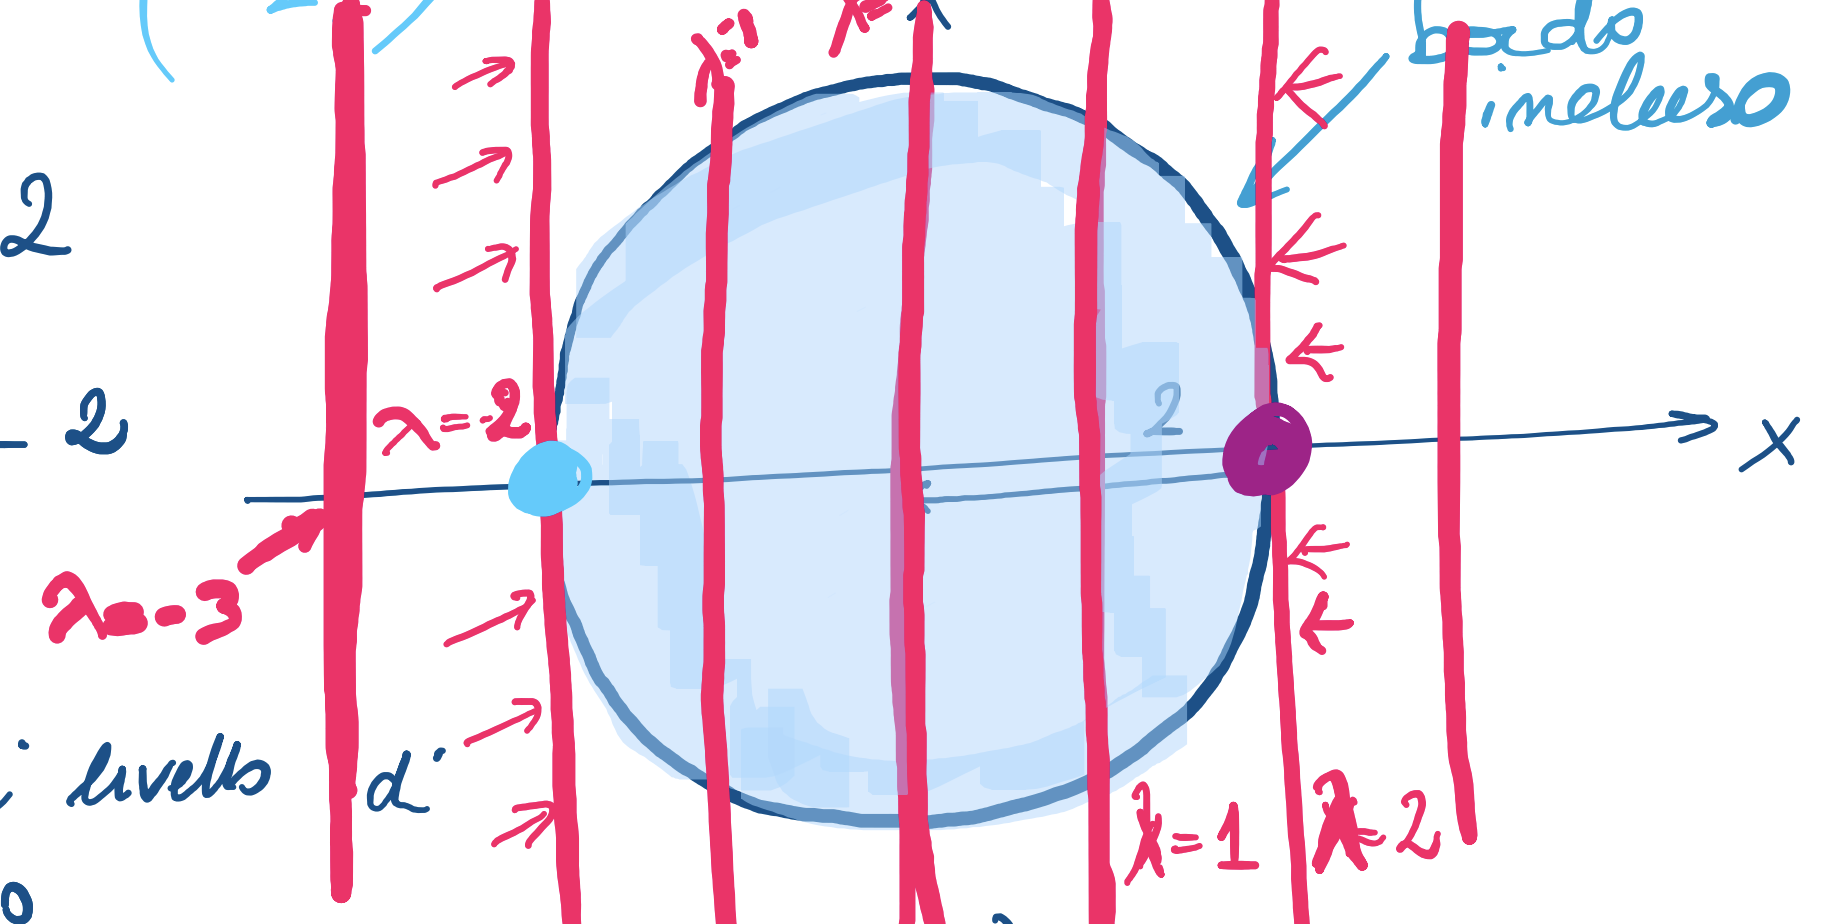
\includegraphics[width=4.7cm]{images/max-min-ess-insiemi-livello-1.png}
\end{wrapfigure}
In questo caso ci aspettiamo che il punto di massimo sia $(2,0)$ e il minimo $(-2, 0)$ quindi $max(f) = 2$ e $min(f) = -2$.\\
Le linee di livello di $f(x,y)$ sono $\{(x,y) \in \mathbb{R}^2 \::\: f(x,y) = \lambda\} = \{(x,y) \in \mathbb{R^2} \::\: x = \lambda\} =$ linee di livello sono rette parallele all'asse y.
\begin{itemize}
    \item Si può osservare in questo esempio che il massimo di $f(x,y)$ in A è il più grande $\lambda$ tale che $A \cap \{(x,y) \::\: f(x,y) = \lambda\} \neq \O$, in questo caso è $\lambda = 2$ che è il massimo di f.
    \item Mentre il minimo di $f(x,y)$ in A è il più piccolo $\lambda$ tale che $A \cap \{(x,y) \:\: f(x,y) = \lambda\}\neq \O$, quindi in questo caso $\lambda = -2$ e quindi $min(f) = -2$.
\end{itemize}
\hspace{-15pt}Possiamo riassumere questo metodo dicendo che andiamo a cercare il più grande e il più piccolo $\lambda$ per i quali l'insieme di livello $\lambda$ interseca A.

\begin{example}
Dato $f(x,y) = 2x-y$ e $A =$ triangolo con vertici $(0,0), (0,1), (3,2)$. 
\end{example}

\begin{wrapfigure}[9]{l}{5.3cm}
    \vspace{-10pt}
    \centering
    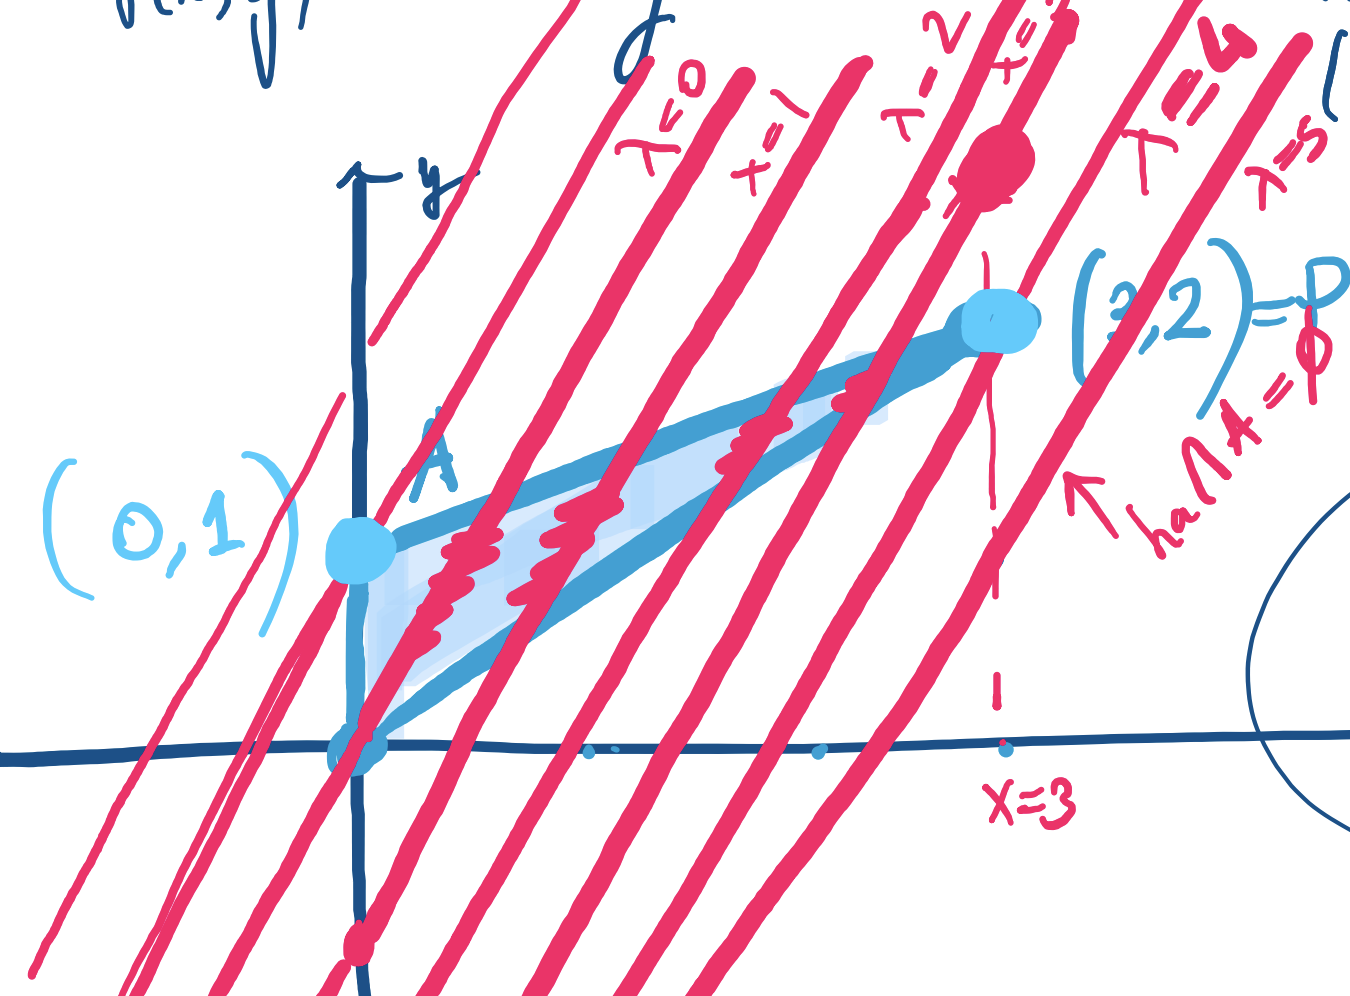
\includegraphics[width=4.5cm]{images/max-min-ess-insiemi-livello-2.png}
\end{wrapfigure}
$f$ continua si A e compatto quindi per Weirstrass esiste sia massimo che minimo in $f$. In questo caso il metodo intuitivo non è fattibile quindi si usa le linee di livello, sappiamo che $\{(x,y) \in \mathbb{R}^2 \::\: f(x,y) = \lambda\} = \{(x,y) \in \mathbb{R}^2 \::\: 2x-y = \lambda\}$ linee di livello $\lambda$. Se $\lambda = 2$ ho $y = 2x -2$, con $\lambda = 3$ ho $y = 2x -3$ (in questo caso ancora la retta interseca il triangolo), con $\lambda = 4$ ho $y = 2x - 4$ per $x = 3$ ho $y= 2 \cdot 3 - 4 = 2$ retta passante per $(3,2)$, se $\lambda$ più grande per cui l'insieme dato A interseca le linee di livello $\lambda$ è $\lambda = 4$ quindi per il metodo delle linee di livello $max(f) = 4$ che il punto $(3,2)$.\\\\
Per il punto minimo si procede analogamente ma con $\lambda$ più piccoli, possiamo vedere in questo caso che $\lambda = -1$ è il pià piccolo $\lambda$ tale che $\{$linee di livello $\lambda\} \cap A \neq 0$, quindi $min(f) = -1$ ed il punto di minimo è $(0,1)$.

\begin{example}
Consideriamo la funzione $f(x,y) = x^2 + y^2$ su $A = [2,5] \times [-1,1]$, anche in questo caso f è continua su A compatto quindi esistono massimo e minimo.
\end{example}
\begin{wrapfigure}[6]{l}{5.3cm}
    \vspace{-10pt}
    \centering
    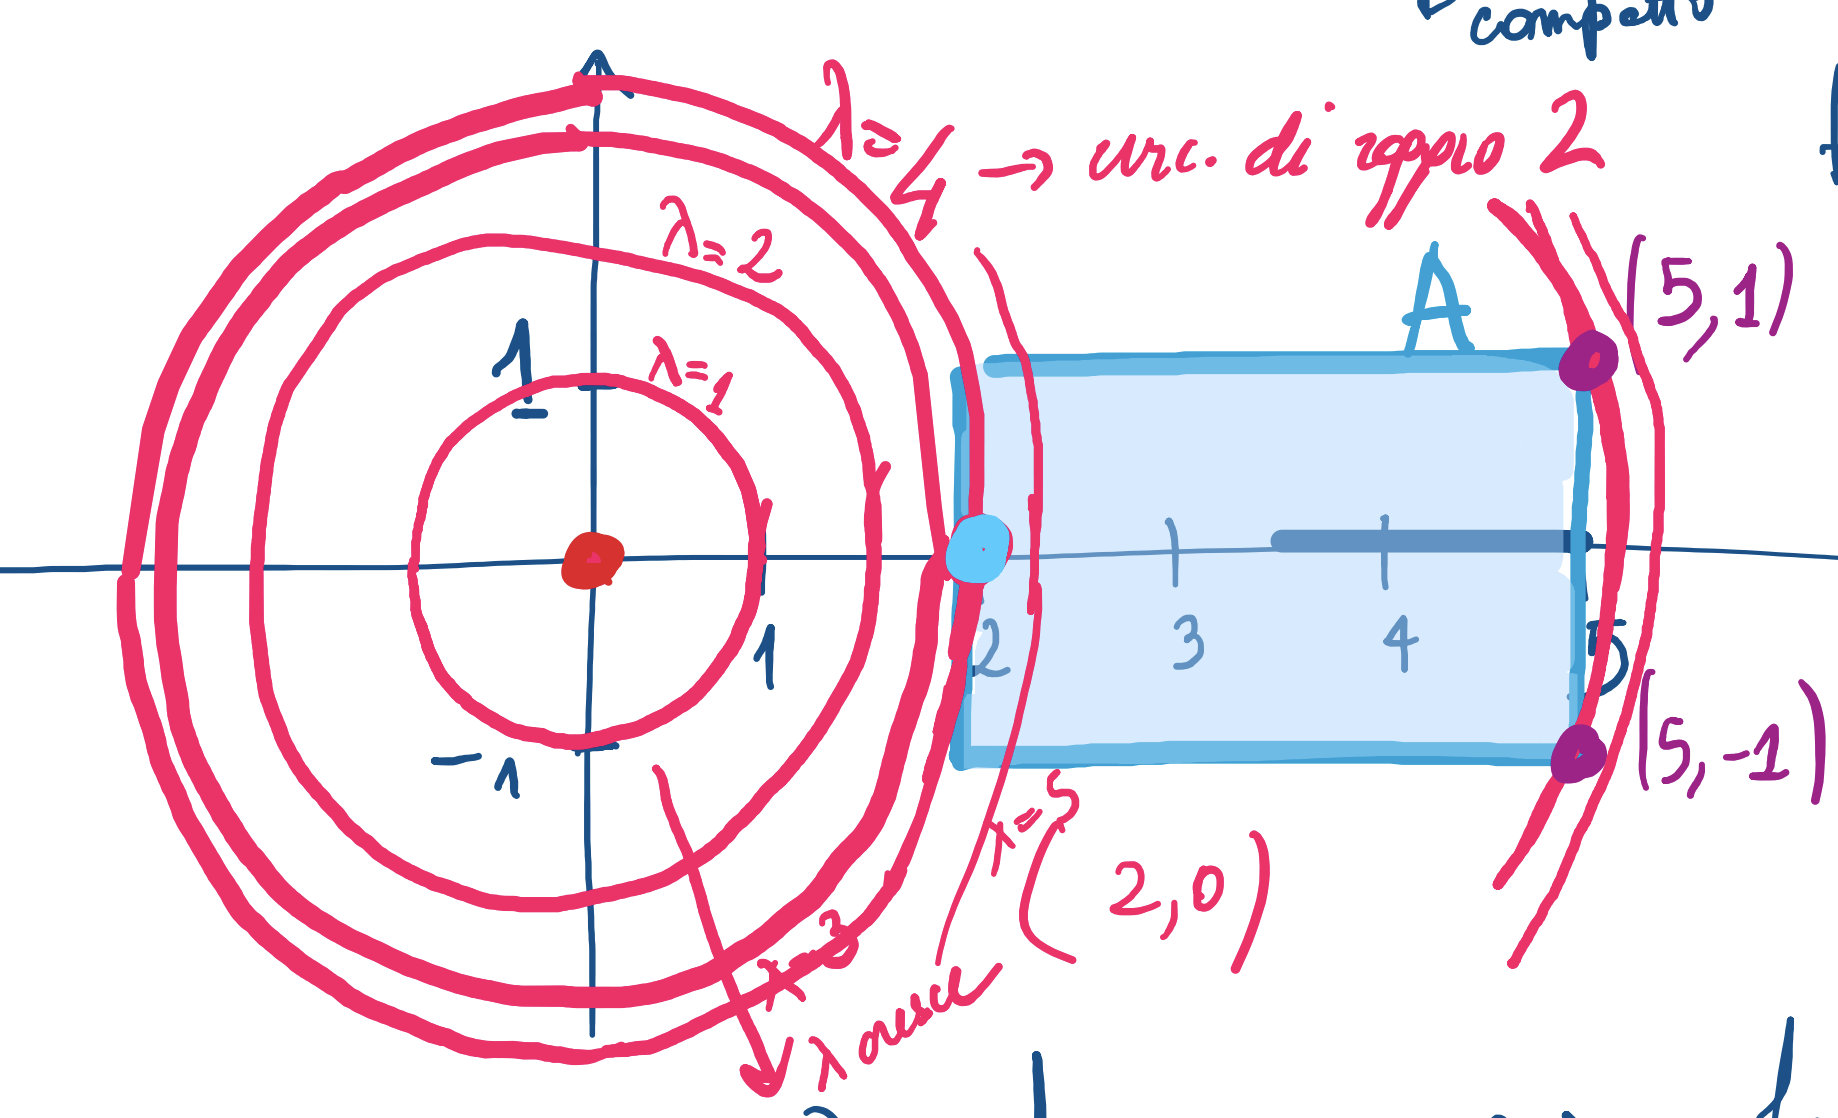
\includegraphics[width=4.5cm]{images/max-min-ess-insiemi-livello-3.png}
\end{wrapfigure}
Le linee di livello $\lambda$ sono circonferenze con centro nell'origine e raggio $\sqrt{\lambda}$. Il $\lambda$ più piccolo tale che $L_{\lambda} \cap A \neq \O$ è $\lambda = 4$ quindi $min(f) = 4$. I punti di coordinate $(5,1)$ e $(5,-1)$ sono tali che $5^2 + 1^2 = 26$ quindi $L_{26} \cap A = (5,1) \cup (5,-1)$, quindi 25 è il $\lambda$ più grande tale che $L_{\lambda} \cap A \neq \O$ quindi $max(f) = 26$ e i punti di max sono due $(5,1)$ e $(5,-1)$.\\

\subsubsection{Metodo di parametrizzazione}
Per capire questo metodo rifacciamo l'esercizio visto sopra usando appunto questa metodologia di risoluzione.
\begin{example}
Data $f(x,y) = x^2 + y^2$, $A = [2,5] \times [-1,1]$. Questo metodo ci dice che bisogna cercare i punti max e min in varie categorie.
\begin{itemize}
    \item Punti stazionari interi, interni perché $(x_0,y_0) \in (2,5) \times (-1,1)$ e $\nabla f(x_0,y_0) = 0$. Nel nostro caso $\nabla f = (2x, 2y)$ che si annulla soltanto se $(x,y) = (0,0)$, ma (0,0) non è punto interno di A quindi non ci sono punti interni stazionari.
    \item Punti singolari interi, che sono quelli in cui la funzione non è differenziabile. Nel nostro caso $f(x,y) = x^2 + y^2$ è differenziabile su tutto A, quindi non abbiamo punti singolari interni.
    \item Punti di bordo. Per cercare questi punti ci sono vari metodi, uno di questi è il \textbf{metodo della parametrizzazione}, ocn questo metodo parametrizzo i vari pezzi del bordo, e così facendo vedo la funzione come si comporta rispetto questi pezzi.
    \begin{enumerate}
        \item $\{(t,1) \:\: t \in [2,5]\}$, quindi $g_1(t) = f(t,1) = t^2 +1$.
        \item $\{(5,t) \::\: t \in [-1,1]\}$, quindi $g_2(t) = f(5,t) = t^2 + 25$.
        \item $\{(t,-1) \::\: t \in [2,5]\}$, quindi $g_3(t) = f(t,-1) = t^2 + 1$.
        \item $\{(2,t) \::\: t \in [-1,1]\}$, quindi $g_4(t) = f(2,t) = t^2 + 4$.
    \end{enumerate}
    Adesso studio le 4 funzioni sopra definite ed ho per ciascuna dei massimi e dei minimi su ogni tratto, poi li confronto e rendo il più piccolo ed il più grande che corrispondono al minimo ed al massimo.
    \begin{enumerate}
        \item Minimo per $t=2$ e massimo per $t = 5$.
        \item Minimo per $t=0$ e massimo per $t = \pm 1$.
        \item Minimo per $t=2$ e massimo per $t = 5$.
        \item Minimo per $t=0$ e massimo per $t = \pm 1$.
    \end{enumerate}
    Quindi concludo che $(2,0)$ è minimo e che $(5,-1)$ e $(5,1)$ è il punto di massimo.
\end{itemize}
\end{example}

\begin{example}
Prendiamo $f: \mathbb{R}^2 \to \mathbb{R}$, $f(x,y) = 3x^2 - y + 3$ sull'insieme $A = \{(x,y) \in \mathbb{R}^2 \::\: x^2 - 1 \leq y \leq 3\}$, A è compatto (essendo sia chiuso che limitato), $f$ è continua su un compatto quindi $f$ ammette max e min per Weirstrass.
\end{example}
\begin{wrapfigure}[6]{r}{5cm}
\vspace{-20pt}
    \centering
    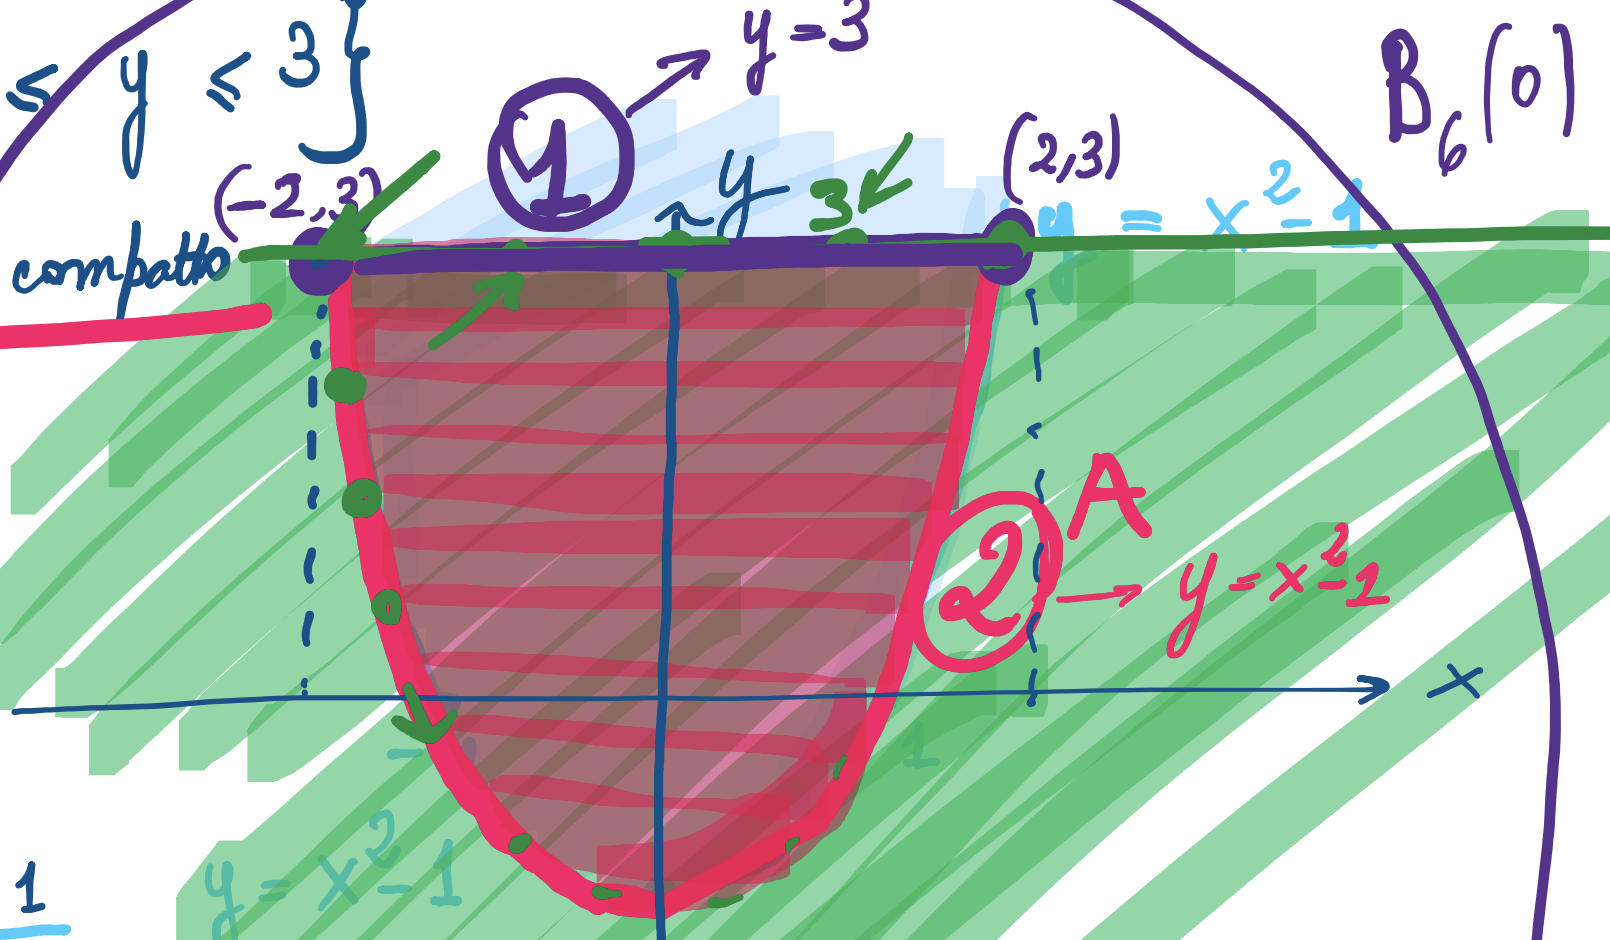
\includegraphics[width=4.5cm]{images/ess-max-min-classico-R2.png}
\end{wrapfigure}
In questo caso le linee di livello tali che $3x^2 - y + 3 = \lambda$, $y = 3x^2 + (x+3)$ non sono un metodo semplice da attuare, quindi optiamo per il metodo classico:
\begin{itemize}
    \item Calcoliamo i punti stazionari interni $\nabla f = 0$, che quindi è $\nabla f(x,y) = (\frac{\partial f}{\partial x}(x,y), \frac{\partial f}{\partial y}(x,y)) = (6x, -1)$ ma $(6x,-1) \neq 0$ perché $-1$ è sempre diverso da 0, quindi non esistono punti stazionari interne quindi non esistono max e min tra i punti interni non singolari di A.
    \item Punti singolari interni non esistono quindi non esistono max e min tra i punti interni di A.
    \item Punti di bordo, andiamo ad usare la parametrizzazione. 
    \begin{enumerate}
        \item Punti di bordo sono quelli che (1) stanno sulla retta $y = 2$ quindi posso porre $x^2 -1 = 3$ quindi $ x = \pm 2$ e quindi abbiamo come punti $(-2,3)$ e $(2,3)$, per parametrizzarlo chiamo $x = t$ e $y = 2$ quindi i punti di tipo (1) sono $(x,y) = (t,3)$ con $t = [-2,2]$. Quindi la funzione $f$ rispetto a (1) possiamo chiamarla $g_1(t) = f(t,3)$ con $t \in [-2,2]$ è $g_1(t) = 3t^2$.
        \item Abbiamo poi i punti che stanno sulla parabola $y = x^2 - 1$ per $x \in [-2,2]$ quindi di tipo (2), per parametrizzare questo bordo prendiamo i punti che possono essere scritti come $(x,y) = (t, t^2-1)$ con $t \in [-2,2]$ quindi avendo come parametro $x = t$, su questo secondo bordo definirò $g_2(t) = f(t,t^2-1) = 3t^2 - t^2 + 1+4 = 2t^2+4$.
    \end{enumerate}
    Ho quindi sul bordo (1) $g_1(t) = 3t^2$ e su (2) ho $g_2(t) = 2t^2+4$ per $t \in [-2,2]$, ora dobbiamo cercare i massimi ed i minimi. Per $g_1(t) = 3t2$ ho che:
    \begin{itemize}
        \item Il massimo per $t = -2$ o per $t = 2$ è $g_1(t) = 12$.
        \item Mentre il minimo per $t = 0$ è. $g_1(t) = 0$.
    \end{itemize}
    Invece per $g_2(t) = 2t^2 + 4$ vediamo che:
    \begin{itemize}
        \item Il massimo per $t = -2$ o per $t = 2$ avrò che $g_2 (t) = 12$.
        \item Mentre il minimo come sempre ho $t=0$ con il quale ho $g_2(t) = 4$.
    \end{itemize}
    Avremo dunque come massimo $t=-2$ e $t = 2$ perché abbiamo il valore massimo in entrambi i $g_1, g_2 = 12$, il punto minimo di $f$ è $(0,3)$ e $f(0,3) = g_1(0) = 0$.
\end{itemize}

\hspace{-15pt}Ecco alcuni casi notevoli per andare a parametrizzare i bordi:
\begin{enumerate}
    \item Segmento di estremi $(a_1,b_1)$ e $(a_2,b_2)$. Questi punti possono essere parametrizzati andando a scrivere $(x,y) = (a_1,b_1) + t(a_2-a_1, b_2 - b_1)$ con $t \in [0,1]$.
    \item Il tratto del grafico $y = \varphi(x)$ con $x \in [a,b]$. In generale descriviamo $(x,y) = (t, \varphi(t))$ con $t \in [a,b]$.
    \item La circonferenza con centro in $(0,0)$ e raggio r. Questo caso si parametrizza prendendo $(x,y) = (r \cdot \cos{\Theta}, r \cdot \sin{\Theta})$ con $\Theta \in [0,2\pi]$.
    \item La circonferenza con centro in punto $(x_0, y_0)$ e raggio r. Analogo alla precedente, quindi $(x,y) = (x_0 + r \cdot \cos{\Theta}, y_0 + r\cdot \sin{\Theta})$ con $\Theta \in [0,2\pi]$.
    \item L'ellisse di equazione $ax^2 + by^2 = 1$ con $a,b > 0$. Si parametrizza simile alla circonferenza quindi con $(x,y) = (\frac{1}{\sqrt{a}}\cos{\Theta}, \frac{1}{\sqrt{b}}\sin{\Theta})$ con $\Theta \in [0,2\pi]$.
\end{enumerate}
\subsubsection{Moltiplicatori di Lagrange}
\begin{definition}[Luogo di zeri]
Data una funzione $\varphi: \mathbb{R}^2 \to \mathbb{R}$ allora l'insieme $V = \{(x,y) \in \mathbb{R}^2 \::\: \varphi(x,y) = 0\}$ si dice \textbf{luogo di zeri} della funzione $\varphi$ (linea di livello $\lambda = 0$).
\end{definition}
\hspace{-15pt}Il metodo dei moltiplicatori di Lagrande serve per trovare possibili punti di massimo e minimo di una funzione $f$ su un insieme A quando il bordo di A è un luogo di zeri di una funzione.
\begin{example}
Prendiamo $f(x,y)$ su $A = \{(x,y) \in \mathbb{R}^2 \::\: x^2 + y^2 \leq 3\}$. Il bordo di A è la circonferenza data da $x^2 + y^2 = 3$ (quindi la circonferenza che delimita) questa circonferenza la posso scrivere come $(x,y) \in \mathbb{R}^2$ tali che $x^2 + y^2 - 3 = 0$, se definisco $\varphi(x,y) = x^2 + y^2 -3$ allora il bordo di A è il luogo di zeri della funzione $\varphi$ e quindi posso usare il metodo dei moltiplicatori di Lagrange.
\end{example}

\begin{example}
Se invece prendiamo un insieme $A = \{(x,y) \in \mathbb{R}^2 \::\: 2x^2 + 3y^2 \leq 5\}$, analogamente in questo caso il bordo di A sarà il luogo di zeri della funzione $\varphi = 2x^2 + 3y^2 -5$ perché quando $\varphi (x,y) = 0$ se e solo se è il bordo di A.
\end{example}

\hspace{-15pt}Supponiamo per semplicità di essere in $\mathbb{R}^2$ e supponiamo che V sia il luogo di zeri di $\varphi(x,y)$, allora i candidati ad essere punti di minimo o massimo di $f$ in V si cercano tra le seguenti due categorie.
\begin{enumerate}
    \item Punti $(x,y) \in \mathbb{R}^2$ tali che $\begin{cases}\varphi(x,y) = 0\\ \nabla \varphi(x,y) = 0\end{cases}$ Quindi se esiste un punto che soddisfa questo sistema (1) allora tale punto è candidato a punto di massimo e minimo.\\
    In questo caso (con $\mathbb{R}^2$) ho 3 condizioni perché bisogna determinare che la derivata sia rispetto a x che y sia 0, con più variabili aumentano anche il numero di condizioni.
    \item Punti $(x,y) \in \mathbb{R}^2$ tali che $\begin{cases}\varphi(x,y) = 0 \\ \nabla f(x,y) = \lambda \nabla \varphi(x,y) \text{ per }\lambda \in \mathbb{R}\end{cases}$ Deve quindi accadere che il gradiente di $f$ è un multiplo del gradiente di $\varphi$. Anche in questo caso dobbiamo risolvere una sistema di 3 equazioni perché dobbiamo verificare sia la derivata rispetto a x che rispetto a y, cerco quindi in questo caso $\lambda, (x,y)$ tali che (2) valga, e quindi in questo caso 3 equazioni per 3 incognite che è più semplice da risolvere. (Il numero $\lambda$ si dice moltiplicatore di Lagrange)
\end{enumerate}

\begin{example}
Consideriamo la funzione $f(x,y) = x - 2y$ e come insieme $A = \{(x,y) \in \mathbb{R}^2 \::\: x^2 + y^2 \leq 3\}$, $f$ continua su A quindi esiste massimo e minimo. Proviamo come prima cosa proviamo ad utilizzare il metodo classico per la ricerca dei massimi e i minimi, quindi cerchiamo i punti stazionari interni, i punti singolari interni e i punti di bordo.
\begin{enumerate}
    \item Punti stazionari interni. Il gradiente è $\nabla f(x,y) = (1,-2)$ che è costante e quindi possiamo vedere che non ci sono punti stazionari interni.
    \item Punti singolari interni. Dal caso prima possiamo anche dire che non ci sono punti singolari interni.
    \item Punti di bordo. I punti del bordo sarà l'insieme $V = \{(x,y) \in \mathbb{R}^2 \::\: x^2 + y^2 = 3\}$, V è luogo di zeri di $\varphi = x^2 + y^2 - 3$ se $(x,y) \in V \Longleftrightarrow \varphi(x,y) = 0$, andiamo allora ad utilizzare il metodo dei moltiplicatori di Lagrange per cerare i punti di max e min sul bordo.\\
    \begin{enumerate}
        \item Come prima cosa dobbiamo trovare i punti $(x,y)$ tali che $\begin{cases}\varphi(x,y) = 0\\ \nabla \varphi(x,y) = 0\end{cases}$.\\
        Abbiamo già che $\varphi(x,y) = x^2 + y^2 -3$ quindi andiamo a calcolare il gradiente $\nabla \varphi(x,y) = (2x, 2y)$. Possiamo ora scrivere la condizione come $\begin{cases}x^2 + y^2 -3 = 0\\ 2x=0 \\ 2y = 0\end{cases}$ le ultime due però sono incompatibili con la prima e quindi non esistono soluzioni per questo sistema.
        \item Ora dobbiamo provare a trovare soluzioni nel sistema $\begin{cases}\varphi(x,y) = 0 \\ \nabla f(x,y) = \lambda \nabla \varphi(x,y)\end{cases}$, quindi cerco $\lambda,x,y$ tali che questo sistema sia verificato. Quindi risolviamo\\\\
        $\begin{cases}x^2 + y^2 - 3 = 0 \\ 1 = \lambda (2x) \\ -2 = \lambda(2y)\end{cases} = \begin{cases}x = \frac{1}{2x} \\ y = -\frac{1}{\lambda} \\ \frac{1}{4x^2} + \frac{1}{\lambda^2} - 3 = 0\end{cases} = \begin{cases}x = \frac{1}{2x} \\ y = -\frac{1}{\lambda} \\ 1 + 4 = 3 \cdot 4 \lambda^2\end{cases}$\\\\
        l'ultima equazione è uguale a $5 = 12\lambda^2 \Longrightarrow \lambda^2 = \frac{5}{12} \Longrightarrow \lambda = \pm \frac{\sqrt{5}}{2\sqrt{3}}$, allora ho le soluzioni\\
        $\begin{cases}\lambda = \frac{\sqrt{5}}{2\sqrt{3}} \\ x = \frac{\sqrt{3}}{\sqrt{5}} \\ y = -\frac{2\sqrt{3}}{\sqrt{5}}\end{cases}$ e $\begin{cases}\lambda = -\frac{\sqrt{5}}{2\sqrt{3}} \\ x = -\frac{\sqrt{3}}{\sqrt{5}} \\ y = \frac{2\sqrt{3}}{\sqrt{5}}\end{cases}$ Quindi ho 2 soluzioni al sistema (2 terne di soluzioni).\\
        I candidati punti di massimo e minimo di $f$ sul bordo $P_1 = (\frac{\sqrt{3}}{\sqrt{5}}, -\frac{2\sqrt{3}}{\sqrt{5}})$ e $P_2 = (-\frac{\sqrt{3}}{\sqrt{5}}, \frac{2\sqrt{3}}{\sqrt{5}})$, per ora sapere qualche è il massimo e quale è il minimo dovrò valutare $f(P_1) = \frac{\sqrt{3}}{\sqrt{5}} + \frac{4\sqrt{3}}{\sqrt{5}} = \frac{5 \sqrt{3}}{\sqrt{5}} = \sqrt{15}$ che è il max e $f(P_2) = -\frac{\sqrt{5}}{\sqrt{5}} - \frac{4\sqrt{5}}{\sqrt{5}} = -15$ che è il min.\\
        Quindi $P_1$ e punto di massimo e $P_2$ è punto di minimo.
    \end{enumerate}
\end{enumerate}
\end{example}
\begin{wrapfigure}[8]{l}{6cm}
\vspace{-10pt}
    \centering
    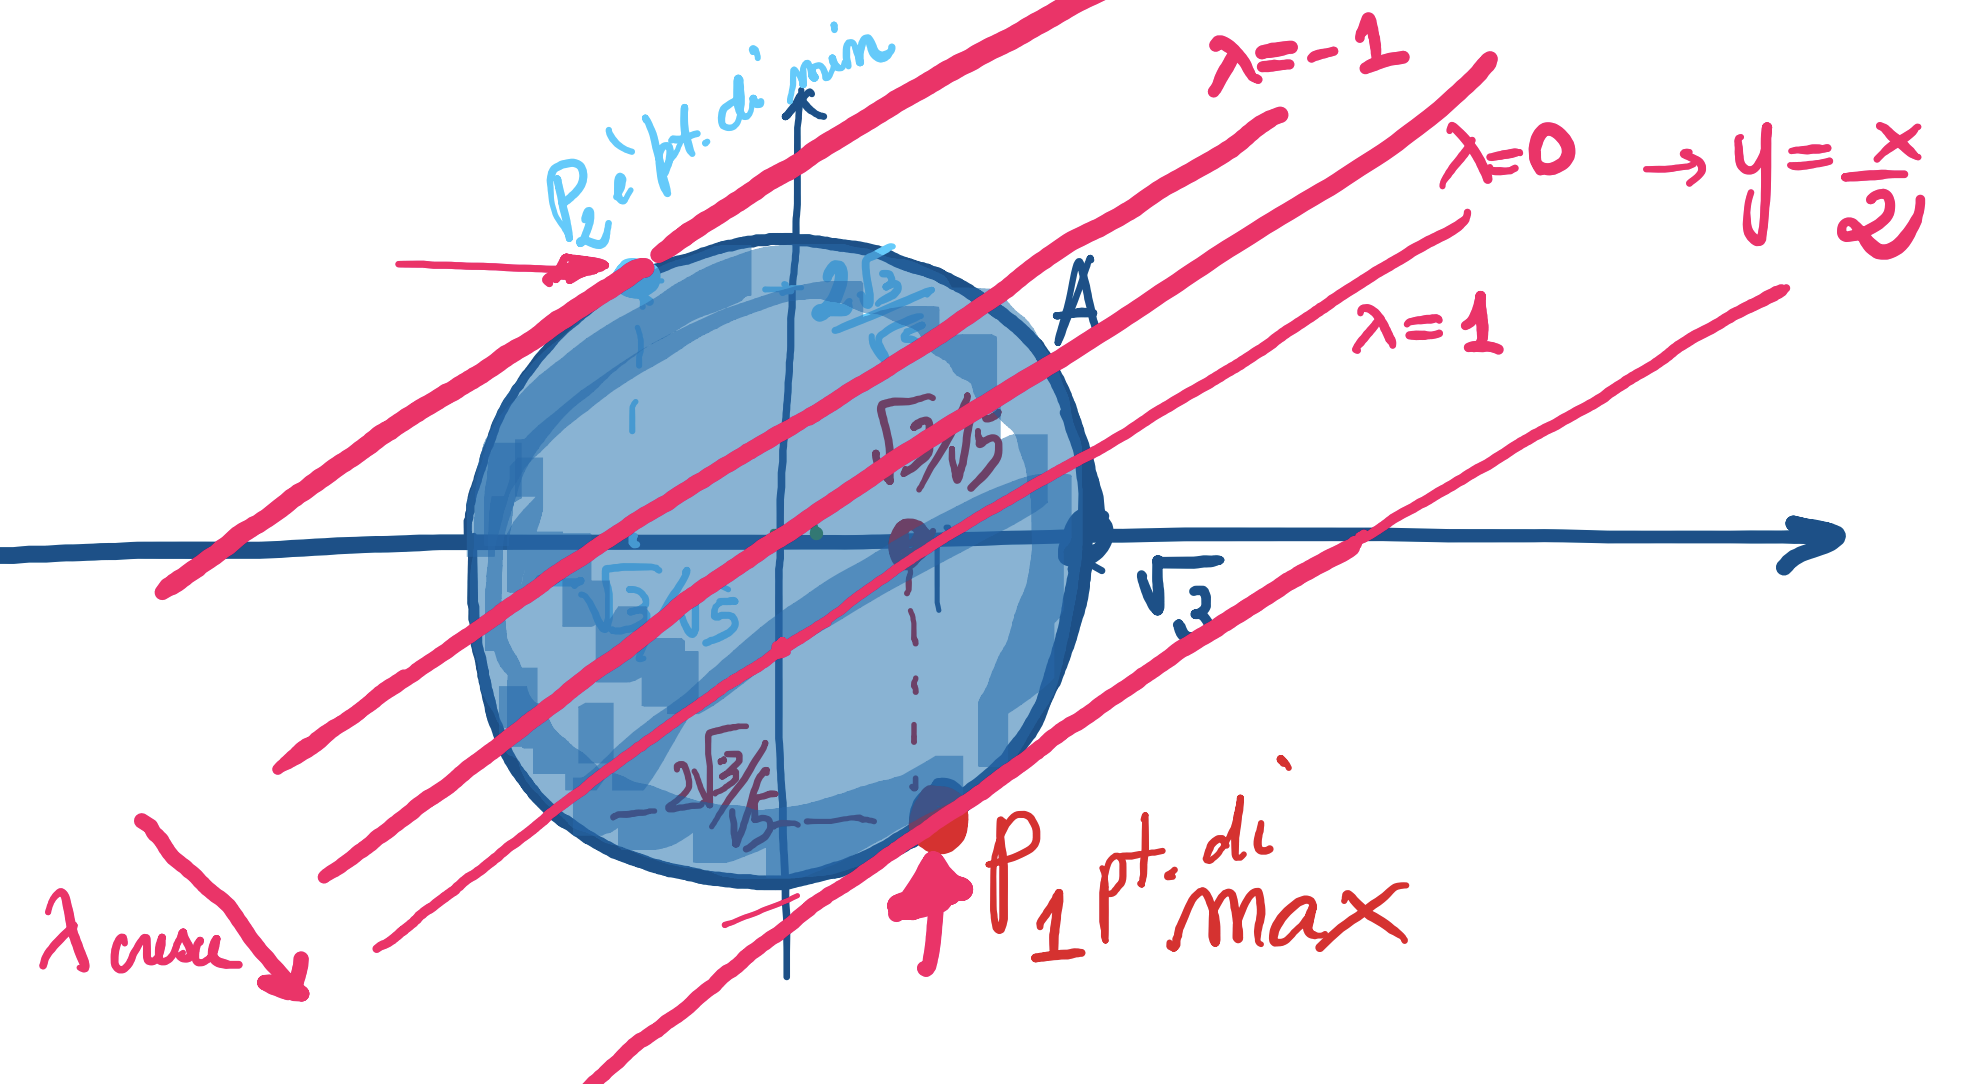
\includegraphics[width=5.5cm]{images/ess-moltip-lagrange-1.png}
\end{wrapfigure}
Possiamo ora chiederci se avessimo usato il metodo delle linee di livello avremmo ottenuto lo stesso risultato. Tramite questo metodo abbiamo la linee di livello $\{(x,y) \in \mathbb{R}^2 \::\: x - 2y = \lambda\}$ ovvero $2y = x - \lambda$ oppure $y = \frac{x}{2} - \frac{\lambda}{2}$, quindi le linee di livello sono con $\lambda = 0 \to y = \frac{x}{2}$, con $\lambda = 1 \to y = 1 \to y = \frac{x}{2} - \frac{1}{2}$ e con $\lambda = -1 \to y = \frac{x}{2} + \frac{1}{2}$, possiamo vedere come infatti esce una soluzione analoga ma più complessa. \\

\begin{example}
Consideriamo la funzione $f(x,y) = x \cdot y^2$
\end{example}

\begin{wrapfigure}[4]{r}{6cm}
    \vspace{-30pt}
    \centering
    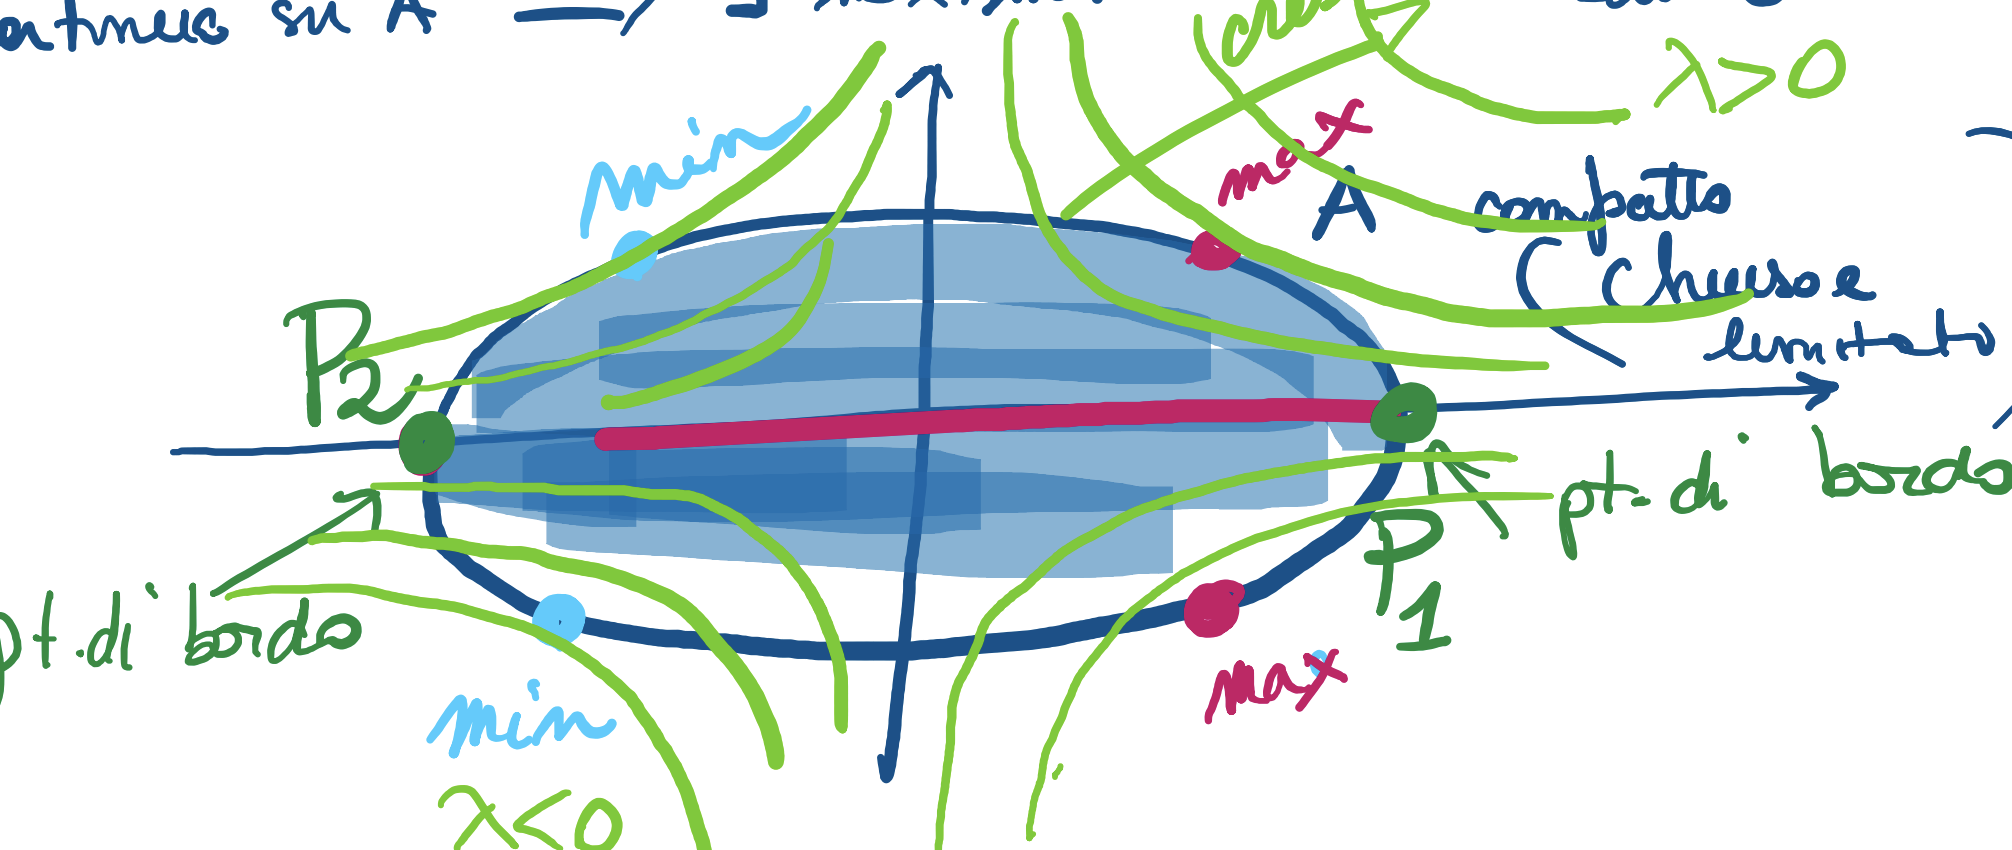
\includegraphics[width=5.5cm]{images/ess-moltip-lagrange-2.png}
\end{wrapfigure}
\hspace{-15pt}e $A = \{(x,y) \in \mathbb{R}^2 \::\: x^2 + 3y^2 \leq 5\}$, 
A è compatta e $f$ è continua su A quindi esistono massimo e minimo.\\

Andiamo ora a cercare max e min con il metodo classico.
\begin{itemize}
    \item Punti stazionari interni, $\nabla f(x,y) = (y^2, 2xy)$ vediamo ora i punti dove il gradiente si annulla $\nabla f(x,y) = 0$ quindi $y^2 = 0$ e $2xy = 0$ che fa si che $y = 0$, in tutti questi punti $f(x,0) = 0$.
    \item Punti singolari interni non esistono perché il gradiente sull'ellisse considerata non hanno problemi.
    \item Punti di bordo. Punti in cui $\varphi(x,y) = 0$, dove $\varphi(x,y) = x^2 + 3y^2 - 5$, per risolverlo usiamo il metodo dei moltiplicatori di lagrange.
    \begin{enumerate}
        \item Prima proviamo il sistema $\begin{cases}\varphi(x,y) = 0 \\ \nabla \O = 0\end{cases} \Longleftrightarrow \begin{cases}x^2 + 3y^2 - 5 = 0 \\ 2x = 0 \\6y = 0\end{cases}$ dove possiamo vedere che $x = 0$ e $y = 0$ ma questo è incompatibile con la prima equazione quindi questo sistema non ha soluzioni.
        \item Usiamo il secondo sistema \\
        $\begin{cases}\varphi(x,y) = 0 \\ \nabla f(x,y) = \lambda \nabla \varphi(x,y)\end{cases} = \begin{cases}x^2 + 3y^2 -5 = 0\\ y ^2 = 2 \lambda x \\ 2xy = 6 \lambda y\end{cases} = \begin{cases}x^2 + 3y^2 - 5 = 0 \\ xy = 3\lambda y \\ y?2 = 2 \lambda x\end{cases}$ dalla seconda equazione posso ricavare $y (x - 3\lambda) = 0$ che mi fa ottenere $x = 3 \lambda$ e $y = 0$ con il quale ottengo $\begin{cases}x = 3 \lambda \\ y^2 = 2 \lambda \cdot (3 \lambda) = 6 \lambda^2 \\ 9\lambda^2 + 18\lambda^2 = 5\end{cases} = \begin{cases}\lambda^2 = \frac{5}{27} \to \lambda = \pm \frac{\sqrt{5}}{3\sqrt{3}}\\ x = \pm \frac{\sqrt{5}}{\sqrt{3}} \\ y = \pm \sqrt{6}\lambda\end{cases}$ con il quale ottengo 4 punti\\\\
        $P_3 = (\frac{\sqrt{5}}{\sqrt{3}}, \sqrt{6}\frac{\sqrt{5}}{3\sqrt{3}}), P_4 = (-\frac{\sqrt{5}}{\sqrt{3}}, \sqrt{6}\frac{\sqrt{5}}{3\sqrt{3}}), P_5 = (\frac{\sqrt{5}}{\sqrt{3}}, -\sqrt{6}\frac{\sqrt{5}}{3\sqrt{3}}), P_6 = (-\frac{\sqrt{5}}{\sqrt{3}}, -\sqrt{6}\frac{\sqrt{5}}{3\sqrt{3}})$\\\\
        $\begin{cases}y = 0 \\ 2\lambda x = 0 \\ x^2 + 5 = 0\end{cases} = \begin{cases}y = 0 \\ \lambda = 0 \\ x = \pm \sqrt{5}\end{cases}$. Quindi ottengo i due punti $P_1 = (\sqrt{5},0)$ e $P_2 = (-\sqrt{5},0)$.\\\\
    \end{enumerate}
    In totale o quindi 6 punti e da qui dobbiamo calcolare f in questi punti e prendere i massimo per il max ed il minimo per il min. Vediamo così che $f(\frac{\sqrt{5}}{\sqrt{3}}, \pm \frac{\sqrt{10}}{3}) = \frac{10 \sqrt{5}}{9 \sqrt{3}}$ che è il max e $f(-\frac{\sqrt{5}}{\sqrt{3}}, \pm \frac{\sqrt{10}}{3} = -\frac{10\sqrt{5}}{9\sqrt{3}}$ che è il min.
\end{itemize}
Se andassimo a vedere le linee di livello, definite dall'equazione $xy^2 = \lambda$ che possiamo scrivere come $y^2 = \frac{\lambda}{3}$, abbiamo una soluzione analoga a quella con il metodo classico, solo più complessa.


\begin{observation}
Osserviamo che nei punti di massimo o minimo le linee di livello e la linea di bordo (grafico di $\varphi$) sono tangenti. Noi però sappiamo anche che il gradiente è perpendicolare alle linee di livello, e quindi i due gradienti $\nabla f$ e $\nabla \varphi$ saranno paralleli, ecco perché nei punti di massimo e minimo risolviamo il sistema (2) in Lagrange cercando $\nabla f = \lambda \nabla \varphi$.
\end{observation}

\begin{figure}[h!]
\vspace{-10pt}
\centering
\begin{subfigure}{.45\textwidth}
    \centering
    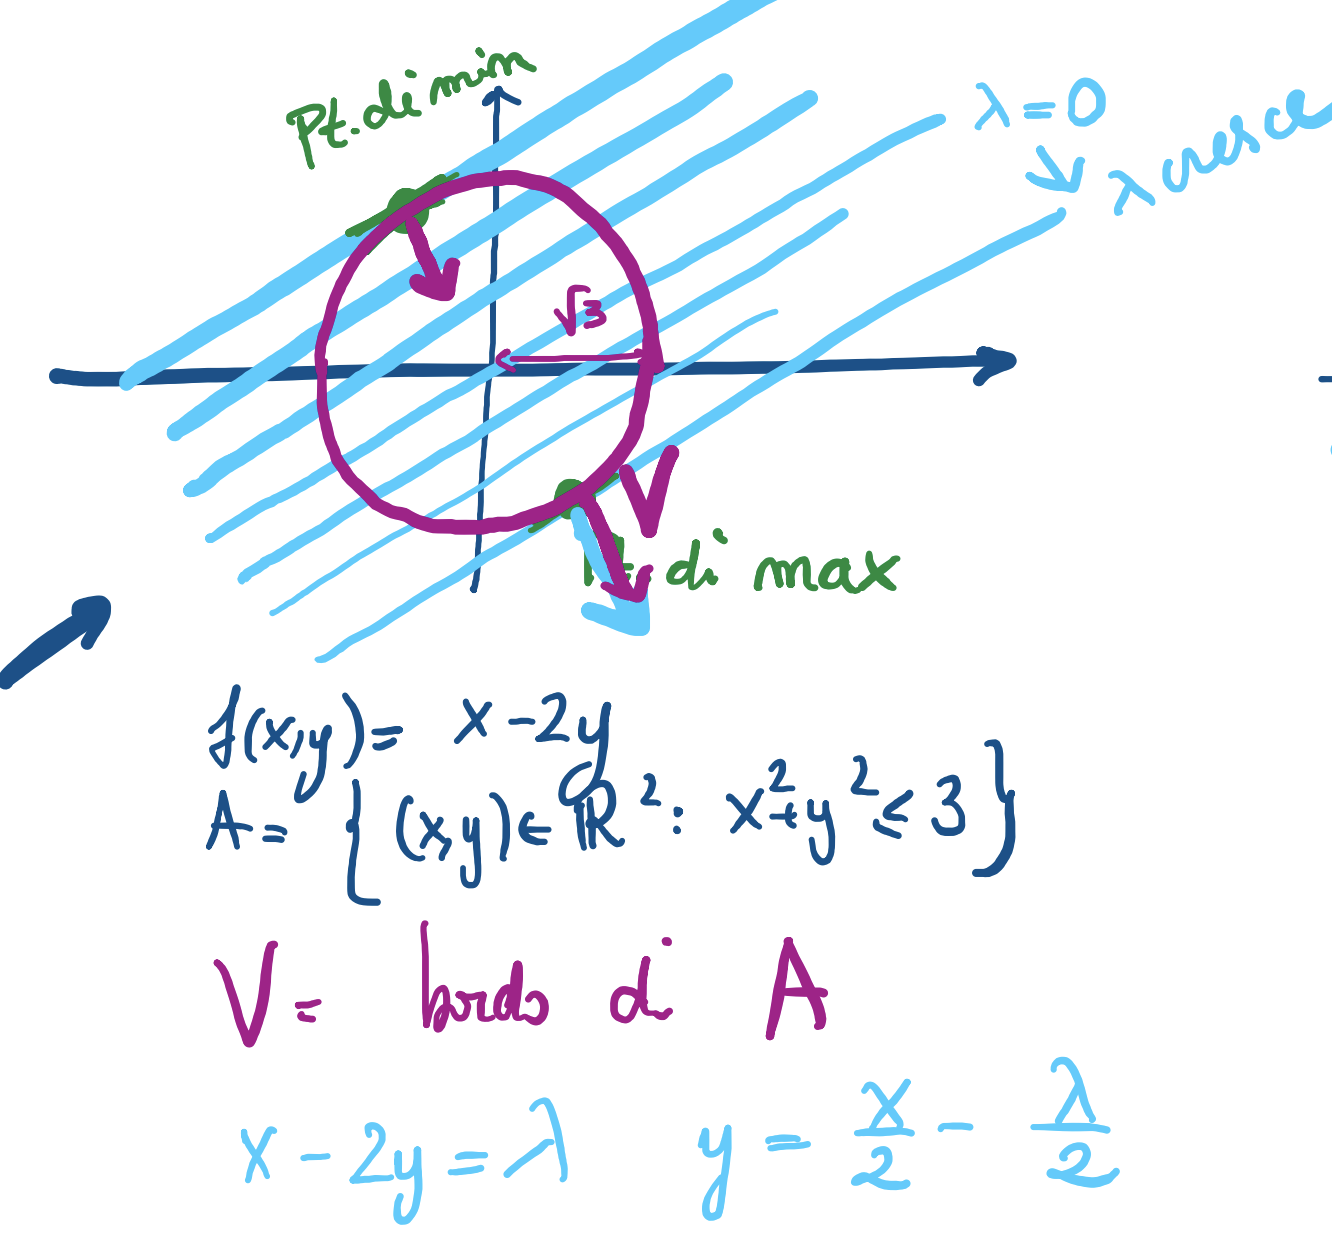
\includegraphics[width=6cm]{images/molt-lagrange-1.png}
\end{subfigure}
\begin{subfigure}{.45\textwidth}
    \centering
    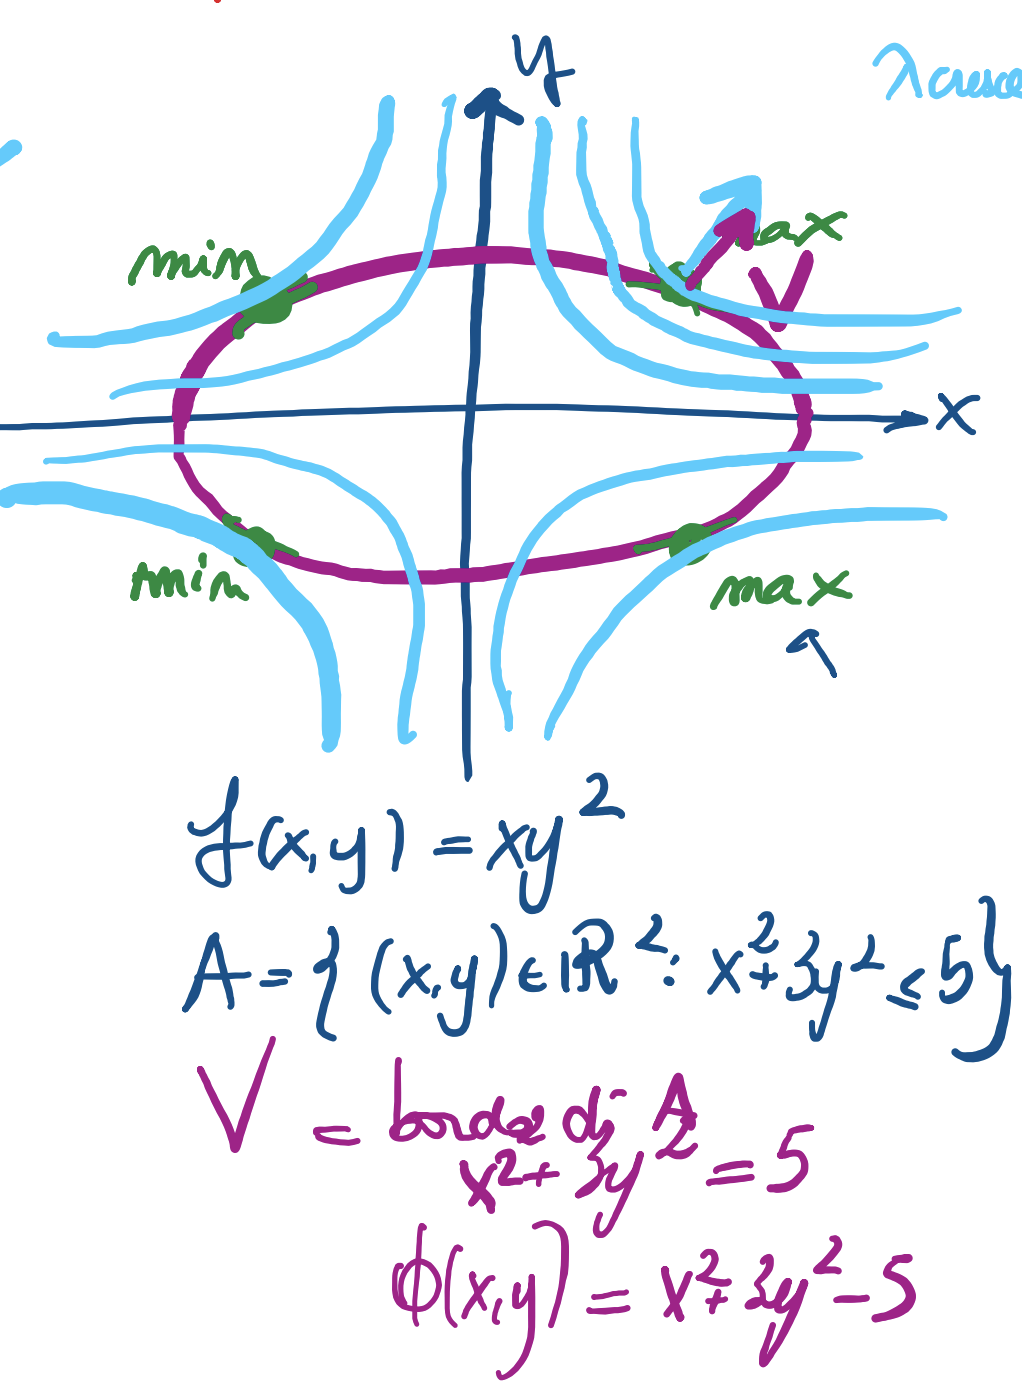
\includegraphics[width=4cm]{images/molt-lagrange-2.png}
\end{subfigure}
\end{figure}
\vspace{-15pt}
\subsubsection{Lagrange geometricamente}
Sia V il bordo di A tale che $f: A \to \mathbb{R}$ con $A \subset \mathbb{R}^2$, supponiamo che $V$ sia il luogo dei zeri di $\varphi(x,y)$, e questo vuol dire che V è linea di livello per $\varphi$.
\begin{enumerate}
    \item Nei punti di massimo e minimo le linee di livello di $f$ e la linea di livello $\lambda=0$ di $\varphi$ sono tangenti (le linee di livello sono tangenti a V nei punti di massimo e minimo).
    \item Sappiamo che $\nabla f$ è sempre perpendicolare alle linee di livello di $f$, e $\nabla \varphi$ è perpendicolare alle linee di livello di $\varphi$ $\Longrightarrow$ i due gradienti devono essere paralleli tra loro.
    \item Quindi $\nabla f$ deve essere un multiplo del $\nabla \varphi \Longrightarrow \nabla f = \lambda \nabla \varphi$.
\end{enumerate}
In conclusione, geometricamente, risolvere il sistema (2) in Lagrange equivale a cercare quei punti di V in cui le linee di livello di $f$ sono tangenti all'insieme di V stesso.\\
Gli esempi in cui il sistema (1) ha soluzioni sono casi molto particolari, vediamo alcuni esempi di questo caso.
\begin{example}
$\varphi(x,y) = x^2 - y^2$, allora $\frac{\partial \varphi}{\partial x}= 2x$ e $\frac{\partial \varphi}{\partial y} = -3y^2$, quindi il sistema (1) è uguale a $\begin{cases}x^2 - y^2 = 0 \\ 2x= 0 \\ -3y^2 = 0\end{cases}$ vediamo che $(x,y) = (0,0)$ è soluzione. Ora però chiediamoci come è fatto V, quindi come è fatto il luogo di zeri di $\varphi$. $V= \{(x,y) \in \mathbb{R}^2 \::\: \varphi(x,y) = 0\}$, $\varphi(x,y) \Longleftrightarrow y^3 = x^2 \Longleftrightarrow y = x^{\frac{2}{3}}$. Il risultato geometrico è una cuspide in cui non so definire la condizione di tangenza.
\end{example}

\begin{example}
Prendiamo $\varphi(x,y) = xy$, $\frac{\partial \varphi}{\partial x} = y$ e $\frac{\partial \varphi}{\partial y} = x$, il sistema (1) è uguale a $\begin{cases}xy = 0\\y = 0\\x=0\end{cases}$ quindi $(0,0)$ è soluzione. $V = \{(x,y) \in \mathbb{R}^2 \::\: xy = 0\}$ corrisponde hai due assi, quindi il punto (0,0) è l'incrocio dei 2 rami. 
\end{example}


\subsection{Teorema di Weristrass generalizzato}
Nell'analisi ad 1 variabile, il teorema di Weristrass generalizzato ci dice che, sia $f: \mathbb{R}\to \mathbb{R}$ continua, supponiamo che $\lim\limits_{x\to -\infty}f(x) = \lim\limits_{x\to +\infty}f(x) = +\infty$ allora esiste $\min\limits_{x \in \mathbb{R}}f(x)$. Quindi questa generalizzazione sta nel fatto che l'insieme è definito in un insieme non compatto, per colmare la mancanza di questa ipotesi dobbiamo fare un ipotesi dei limiti ad $\infty$.\\\\
Ora chiediamoci cosa succede per funzioni $f: \mathbb{R}^n \to \mathbb{R}$. Prima cosa dobbiamo chiederci cosa vuol dire andare all'$\infty$ in $\mathbb{R}^n$, questo vuol dire allontanarsi sempre di più dall'origine cioè che $|x|$ (norma) di $x$ va all'$\infty$. $\lim\limits_{(x,y) \to \infty} \Longleftrightarrow \lim\limits_{x^2 + y^2}\to +\infty \Longleftrightarrow \lim\limits_{|x| \to +\infty} \Longleftrightarrow \lim\limits_{\rho \to \infty}$. Quindi $\lim\limits_{(x,y)\to\infty}f(x,y) = +\infty$ vuol dire che $\forall \: M \in \mathbb{R} \: \exists R > 0$ tale che $f(x,y) \geq 0$ questo $\forall (x,y) \in B_R((0,0))$, quindi in generale se chiamiamo $x \in \mathbb{R}^n$ e $f: \mathbb{R}^n \to \mathbb{R}$ abbiamo che $\lim\limits_{x \to \infty}f(x) = +\infty \Longleftrightarrow \forall \: M \in \mathbb{R}$ (anche molto grande) $\exists \: R > 0$ tale che $f(x) \geq M \: \forall \: x \in B_R(0)^c$ (intorno di $\infty$).\\
Da qui possiamo riformulare il teorema di Weristrass generalizzato nel caso di funzioni in più variabili.
\begin{wrapfigure}[3]{r}{4.5cm}
    \centering
    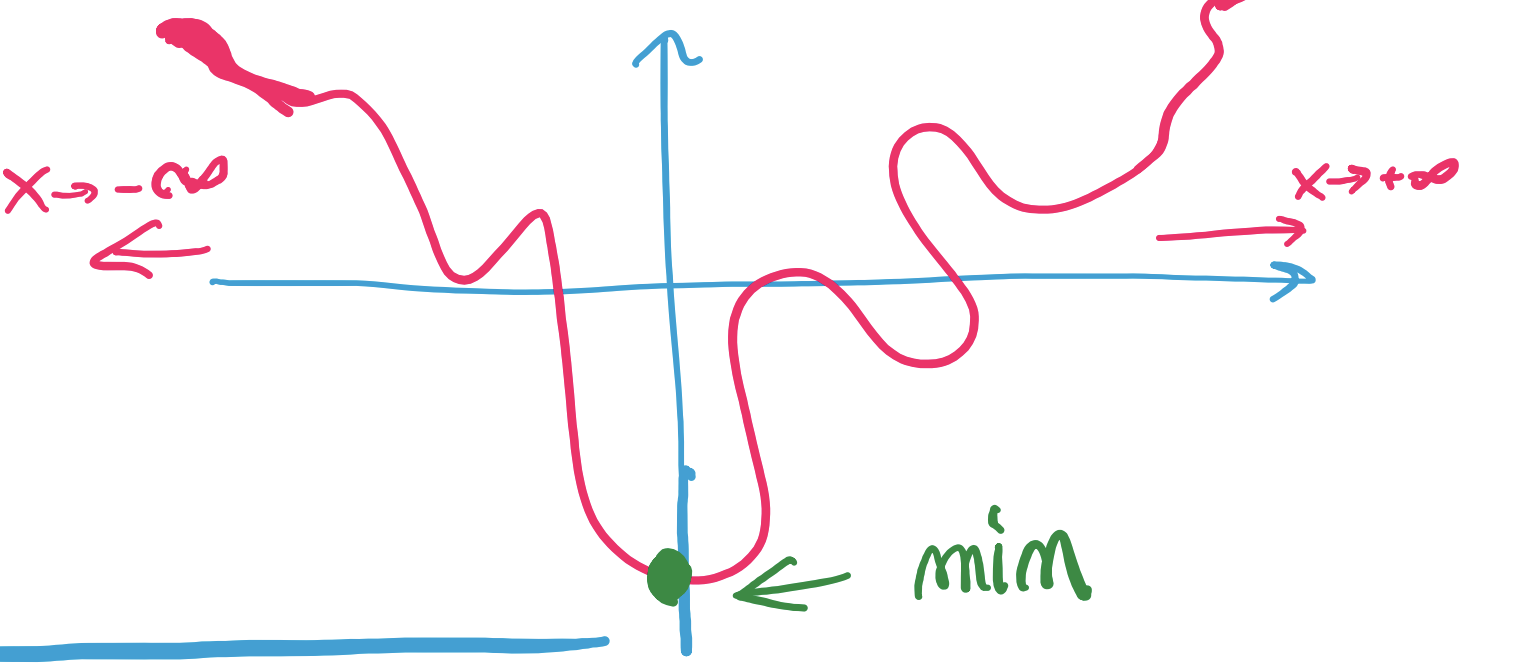
\includegraphics[width=4.2cm]{images/weristrass-generalizzato-R2.png}
\end{wrapfigure}

\begin{definition}[Weristrass generalizzato minimo]
Sia $f: \mathbb{R}^n \to \mathbb{R}$ una funzione continua, e supponiamo che $\lim\limits_{x \to \infty}f(x) = +\infty$ (che vuol dire $\lim\limits_{|x| \to +\infty}f(x) = +\infty$) allora, esiste $\min\limits_{x\in \mathbb{R}^n}f(x)$.
\end{definition}

\begin{demostration}
Sappiamo che $\lim\limits_{|x|\to +\infty}f(x) = +\infty$, quindi da definizione di limite $\forall \: M \exists \: R > 0$ tale che $f(x) \geq M \:\forall \: x \in (B_R(0))^c$, scelgo $f: \mathbb{R}^n \to \mathbb{R}$ uguale a  $M = f(0) + 1$ allora $\exists \: R > 0$ tale che $f(x) \geq f(0) +1 \forall \: x \in (B_R(0))^c$.\\
Considero $f: \overline{B_R(0)} \to \mathbb{R}$ (la linea sopra indica la palla chiusa) con $f: \{x \in \mathbb{R}^n \::\: |x| \leq R\}$ ora questo insieme che è $\overline{B_R(0)}$ è compatto, allora so per Werstrass classico che $\exists \: \min\limits_{x \in \overline{R_R(0)}}f(x) = m$, ora vogliamo dimostra che $m$ è minimo su tutto $R^n$ e non solo su $\overline{B_R(0)}$. Ci sono due casi.
\begin{enumerate}
    \item Se $|x| \leq R$ (dentro la palla), allora $f(x) \geq m$ per definizione di $m = \min\limits_{B_R(0)}f$.
    \item Se $|x| \geq R$ (fuori la palla), allora $f(x) \geq M = f(0) + 1$ (questo per come ho scelto R) $\geq f(0) \geq m$ e questo perché 0 sta nella palla $|x| \leq R$, quindi anche in questo caso $f(x) \geq m$.
\end{enumerate}
Quindi ho dimostrato che $f(x) \geq m \forall \: x \in \mathbb{R}^n$ e per il Teorema di Weristrass classico sappiamo che $\exists \: x_0 \in B_R(0)$ tale che $f(x_0) = m$ quindi ho trovato il minimo su tutto $\mathbb{R}^n$. $\blacksquare$
\end{demostration}

\hspace{-15pt}Tutto questo può essere enunciato in maniera analoga per il massimo di una funzioni in $\mathbb{R}^n$.
\begin{definition}[Weristrass generalizzato massimo]
Sia $f: \mathbb{R}^n \to \mathbb{R}$ una funzione continua, e supponiamo che $\lim\limits_{|x| \to +\infty}f(x) = -\infty$ allora, esiste $\max\limits_{x\in \mathbb{R}^n}f(x)$.
\end{definition}


\section{Derivate parziali seconde}
Nell'analisi in una variabile per studiare localmente una funzione nell'intorno di un punto stazionario, quindi si faceva $f'(x_0) = 0$ e poi su studiava il segno della derivata seconda $f''(x)$ e concludevamo che se $f''(x_0) > 0$ c'era un minimo locale. Nell'analisi in più variabili non possiamo derivare più volte perché non abbiamo una sola variabile, quindi dobbiamo introdurre le derivate successive per funzioni di più variabili.\\\\
La prima cosa che ci verrebbe in mento è quello di derivare parzialmente più volte, quindi avere $\frac{\partial f}{\partial x_1}, \frac{\partial f}{\partial x_2}, \cdots, \frac{\partial f}{\partial x_n}$ con $f: \mathbb{R}^n \to \mathbb{R}$ che sono le derivate parziali prime e, per iniziare, come fare le derivate parziali seconde.

\begin{example}
$f(x,y) = x^2 + y^3 + x^4 \cdot y^5$, $\frac{\partial f}{\partial } = 2x + 4x^3 y^5 = g(x,y)$ e $\frac{\partial g}{\partial y} = 3y^2 + 5x^4 y^4 = h(x,y)$ da qui dobbiamo partire da $g(x,y)$, $h(x,y)$ e ricalcolare le derivate, quindi avrei per esempio per $g(x,y)$ le derivate $\frac{\partial g}{\partial x}$ e $\frac{\partial g}{\partial y}$ che però a loro volta si potrebbero scrivere come $\frac{\partial \partial f}{\partial \partial x} = \frac{\partial^2 f}{\partial x^2} = f_{xx}$ e $\frac{\partial \partial f}{\partial y \partial x} = \frac{\partial^2 f}{\partial y \partial x} = f_{xy}$. Nel caso di $h(x,y)$ invece ho $\frac{\partial h}{\partial x} = \frac{\partial \partial f}{\partial x \partial y} = \frac{\partial^2 f}{\partial x \partial y} = f_{xy}$ e $\frac{\partial h}{\partial y} = \frac{\partial \partial f}{\partial y \partial x} = \frac{\partial^2 f}{\partial y^2} = f_{yy}$.\\
Per questo esempio, ho quindi nel caso di une derivata parziali seconde 4 derivate prime. In maniera più generale $f: \mathbb{R}^n \to \mathbb{R} \Longrightarrow n \cdot n = n^2$ derivate parziali seconde.
\end{example}

\begin{observation}
In generale per una funzioni di n variabili ci sono n derivate parziali prime e $n^2$ derivate parziali seconde. Il metodo di calcolo è sempre lo stesso.
\end{observation}

\begin{example}
Tornando all'esempio scritto sopra ho che $\frac{\partial f}{\partial x} = f_x = 2x + 4x^3 y^5$ che poi va $f_{xx} = 2 + 12x^2y^5$ e $f_{xy} = 20x^3 \cdot y^4$, mentre $\frac{\partial f}{\partial y} = f_y = 3y^2 + 5^4 y^4$ mentre le derivate seconde sono $f_{yy} = 6y + 20x^4y^3$ e $f_{yx} = 20x^3y^4$.
\end{example}

\hspace{-15pt}Vediamo dall'esempio sopra che se derivo $f_{yx}$ e $f_{xy}$ abbiamo due risultati uguali, posso quindi dire che in generale questi valori sono sempre uguali. Da qui possiamo enunciare un teorema che parla dell'ordine di derivazione, enunciamo questo teorema per il caso di $f: \mathbb{R}^n \to \mathbb{R}$.

\begin{theorem}[Inversione dell'ordine di derivazione]
Se $f_{xy}$ e $f_{yx}$ esistono in un intorno del punto $(x_0, y_0) \in \mathbb{R}^n$ e sono continue nel punto $(x_0,y_0)$ allora coincidono ovvero $f_{xy}(x_0,y_0) = f_{yx}(x_0,y_0)$.
\end{theorem}
\hspace{-15pt}Con questo teorema possiamo dire che non conta l'ordine con cui derivo nel calcolare le derivate parziali successive. Questo vale anche per le derivate parziali non solo seconde, ma anche le terze, per esempio $f_{xyx} = f_{yxx}$ e $f_{xyy} = f_{xyy}$.

\subsection{Matrice Hessiana}
Sappiamo che le derivate parziali prime le possiamo derivare in $\nabla f = (f_x, f_y)$, il vettore gradiente e quello che ci da la condizione di stazionarietà di un punto perché corrisponde a $\nabla f(x_0,y_0) = 0$ di $(x_0,y_0)$, le derivate seconde allora le organizzo in una matrice che viene detta \textbf{matrice Hessiana}.
\begin{definition}[Matrice Hessiana]
Si dice \textbf{matrice Hessiana} la matrice formata dalle derivate seconde. Quindi nel caso di $f: \mathbb{R}^2\to \mathbb{R}$ e nel caso di $f: \mathbb{R}^3\to \mathbb{R}$ ho:
\[HF = \begin{bmatrix}f_{xx} & f_{xy} \\ f_{yx} & f_{yy}\end{bmatrix} \hspace{.3cm} e \hspace{.3cm} HF = \begin{bmatrix}f_{xx} & f_{xy} & f_{xz} \\ f_{yx} & f_{yy} & f_{yz} \\ f_{zx} & f_{zy} & f_{zz}\end{bmatrix}\]
\end{definition}

\begin{observation}
Se le derivate parziali seconde esistono e sono continue allora l'ordine di derivazione non importa e HF è simmetrica.
\end{observation}
\hspace{-15pt}L'idea è che tutte le condizioni che in analisi in 1 dimensione coinvolgono il segno della derivata seconda, nell'analisi in pi§ variabili coinvolgono la segnatura della matrice hessiana.

\subsection{Studio di un punto stazionario}
Sia $f: \mathbb{R}^2 \to \mathbb{R}$, ($f: \mathbb{R}^n \to \mathbb{R}$) e sia $(x_0, y_0) \in \mathbb{R}^2$ tale che $\nabla f(x_0, y_0) = 0$ ($\Longleftrightarrow (x_0, y_0)$ punto stazionario), abbiamo i seguenti criteri per decidere se questo punto è minimo o massimo locale.
\begin{enumerate}
    \item Se $Hf = \begin{bmatrix}f_{xx} & f_{xy} \\ f_{yx} & f_{yy}\end{bmatrix}$ (ricordiamo che mettiamo le derivate parziali seconde e che $Hf$ è simmetrica se $f$ è abbastanza regolare, ai sensi del Teorema di inversione di derivazione) è definita positiva allora $(x_0, y_0)$ è punto di minimo locale (una matrice è definita positiva $\Longleftrightarrow$ tutti i suoi autovalori sono positivi (++))
    \item Se $Hf$ è definita negativa (e cioè entrambi gli autovalori sono strettamente negativi $\Longleftrightarrow (--)$) allora $(x_0, y_0)$ è un punto di max locale.
    \item Se $Hf$ è indefinita (quindi se esistono due autovalori discordi $(+-)$) allora $(x_0, y_0)$ è un punto di sella, questo vuol dire che rispetto a questo punto esistono alcune direzione dove la funzione cresce ed altri dove decresce.
    \item Se $Hf$ è degenere (ovvero $det\: Hf = 0$, quindi 0 è tra gli autovalori) non posso concludere niente.
\end{enumerate}

\begin{observation}
La matrice Hessiano fornisce informazioni locali, cioè di permette di concludere l'esistenza di massimo o minimi locali (vicino al punto $(x_0,y_0)$) ma non ci da informazioni globali.
\end{observation}

\hspace{-15pt}Ricordiamo che nell'analisi in 1 dimensione i minimi ed i massimi li avevamo
\begin{itemize}
    \item Se in $f: \mathbb{R}\to \mathbb{R}$ $x_0$ è un punto di minimo locale, allora $f'(x_0) = 0$ e $f''(x_0) \geq 0$ (supponendo che in $x_0 \exists \: f',f''$)
    \item Se $x_0$ è un punto di massimo locale allora $f'(x_0) = 0$ e $f''(x_0) \leq 0$.
\end{itemize}
Nell'analisi in più variabili abbiamo un concetto analogo. Se $f: \mathbb{R}^2 \to \mathbb{R}$ e $(x_0, y_0) \in \mathbb{R}^2$ è punto di minimo locale, allora $\nabla f(x_0, y_0) = 0$ e $Hf(x_0, y_0) \geq 0$ (matrice semi definita positiva, gli autovalori sono non negativi). Nel caso di massimo locale la condizione $\nabla f(x_0, y_0) = 0$ rimane e abbiamo $Hf(x_0, y_0) \leq 0$.\\\\
Riassumendo, condizione sufficiente per un minimo locale è che $\nabla f = 0$ e $Hf > 0$, mentre avere un minimo locale implica che $\nabla f = 0$ e $Hf \geq 0$ (che è condizione necessaria). Analogamente si può dire per il massimo locale.\\
Ad esempio se la matrice hessiana ha autovalori 0,3 ($Hf \leq 0$), posso dire solamente che non è di massimo (perché $Hf \leq 0$).


\begin{figure}[h!]
\vspace{-10pt}
\centering
\begin{subfigure}{.3\textwidth}
    \centering
    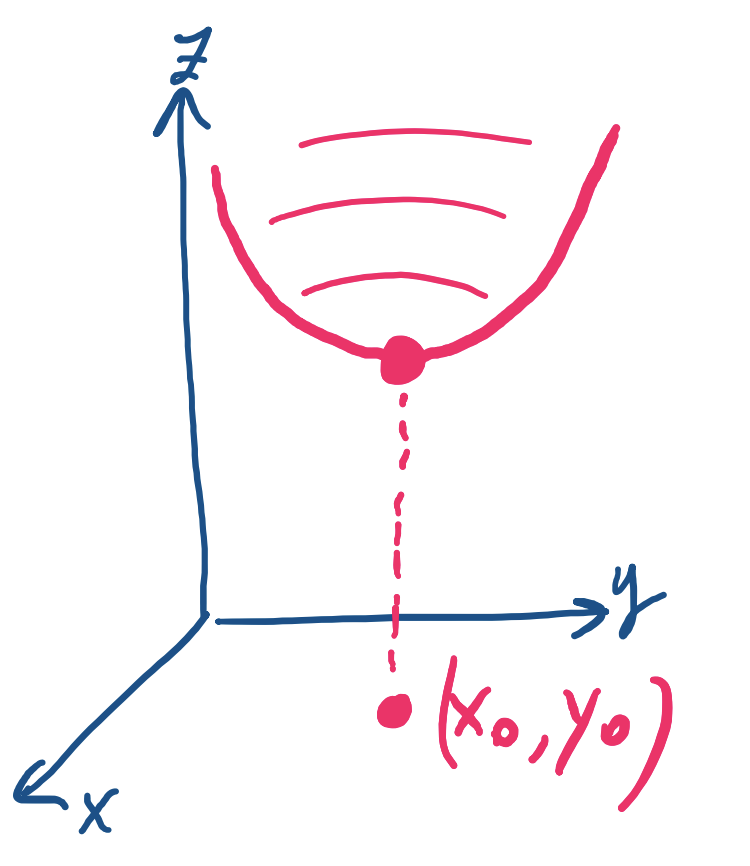
\includegraphics[width=3cm]{images/min-hessiano.png}
    \caption{Minimo}
\end{subfigure}
\begin{subfigure}{.3\textwidth}
    \centering
    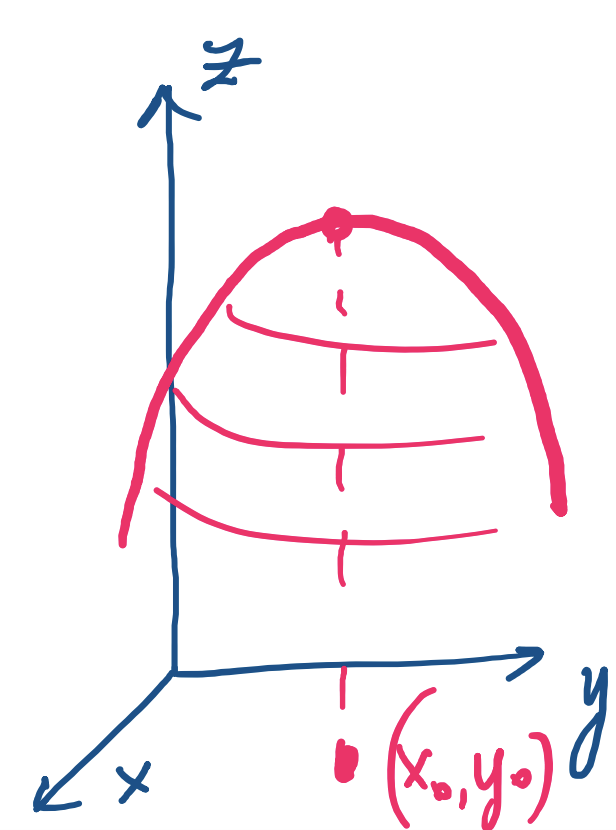
\includegraphics[width=3cm]{images/max-hessiano.png}
    \caption{Massimo}
\end{subfigure}
\begin{subfigure}{.3\textwidth}
    \centering
    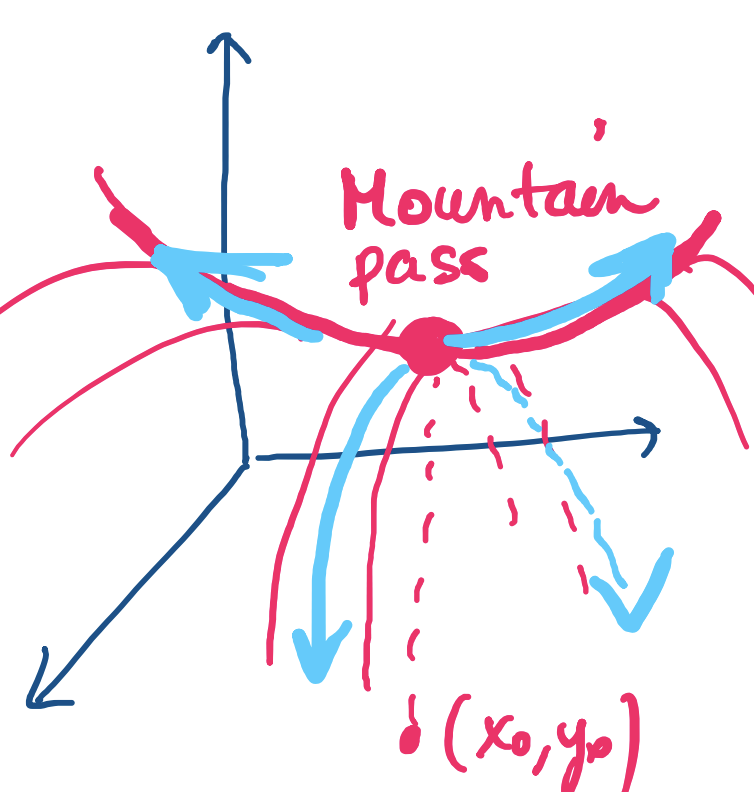
\includegraphics[width=3cm]{images/sella-hessiano.png}
    \caption{Punto di sella}
\end{subfigure}
\end{figure}

\vspace{-10pt}
\begin{example}
Data $f(x,y) = x^2 + y^4$, $(x_0, y_0) = (0,0)$, $\nabla f(x,y) = (\frac{\partial f}{\partial x}(x,y), \frac{\partial f}{\partial y}(x,y)) = (2x, 4y^3)$.\\
$\nabla f(x,y) = 0 \Longleftrightarrow \begin{cases}2x = 0\\ 4y^3 = 0\end{cases} \Longleftrightarrow (x,y) = (0,0) \Longrightarrow (0,0)$ e punto stazionario, per studiare localmente (vicino a (0,0)) la funzione $f$ si calcoliamo la matrice hessiana. $Hf = \begin{bmatrix}f_{xx} & f_{xy} \\ f_{yx} & f_{yy}\end{bmatrix} = \begin{bmatrix}2 & 0 \\0 & 12y^2\end{bmatrix}$, $Hf(0,0) = \begin{bmatrix}2&0\\0&0\end{bmatrix}$, ha un autovalore positivo $\lambda_1 = 2$ ed un autovalore nullo $\lambda_2 = 0$, quindi $Hf$ è semi definita positiva $Hf \geq 0$, l'unica cosa che posso dire è che $(0,0)$ non è un punto di massimo locale, se $(0,0)$ fosse punto di massimo locale infatti avremmo $hf(0,0) \leq 0$. Non possiamo concludere nemmeno se è un minimo perché ci dovrebbe essere un $>$ e non un $\geq$, se però andiamo ad analizzare la funzione vediamo che $f(x) = x^2 + y^4 \geq 0$ e $f(0,0) = 0$ si vede a mano che $(0,0)$ è un punto di minimo globale quindi $f(x,y) > 0 = f(0,0)$ se $(x,y) \neq (0,0)$ con $(x,y) \in \mathbb{R}^2$.
\end{example}

\begin{example}
Consideriamo la funzione $f(x,y) = x^2 - y^4$, anche in questo caso abbiamo che $\nabla f(x,y) = (2x, -4y^3)$, $(0,0)$ è un punto stazionario quindi $\nabla f (0,0) = 0$.\\
$Hf (0,0) = \begin{bmatrix}2 & 0 \\ 0 & 0\end{bmatrix} \geq 0$, gli autovalori sono $\lambda_2 = 2$ $\lambda_2 = 0$ quindi $Hf$ è semi definita positiva in $(0,0)$, quindi il punto $(0,0)$ on è massimo locale. In questo caso l'origine $(0,0)$ non è ne un massimo ne un minimo, questo perché se $y= 0 \to f(x,0) = x^2 \geq 0$ e $x = 0 \to f(0,y) = -y^4 \leq 0$ quindi se mi muovo su l'asse y la funzione cresce mentre su l'asse y la funzione decresce. Vicino a $(0,0)$ esiste punti in cui $f(x,y) > 0$ a punti in cui $f(x,y) < 0$ quindi $(0,0)$ non è ne massimo ne minimo.
\end{example}

\begin{example}
Dato $f(x,y) = x^3 + x^2y^2 + y^4$, $f_x = 3x^2 + 2y^2$, $f_y = 2x^2y + 4y^3$, e $\nabla f = (f_x, f_y)$, quindi $\nabla f(0,0) = 0$ quindi $(0,0)$ è punto stazionario.\\
$Hf(0,0) = \begin{bmatrix}6x + 2y^2 & 4xy \\4xy & 12y^2\end{bmatrix} = \begin{bmatrix}0 & 0 \\ 0 & 0\end{bmatrix}$.
\end{example}

\newpage
\section{Superfici}
Adiamo ora a definire cos'è una superficie in $\mathbb{R}^3$. Per definire queste superfici ci sono 3 approcci, il cartesiano, l'implicito ed il parametrico.

\subsection{Superficie cartesiana}
Consideriamo $A \subset \mathbb{R}^2$ una $f: A \to \mathbb{R}$ la superficie è un grafico di una funzione quindi la possiamo definire come:
\[S = \{(x,y,z) \in \mathbb{R}^3 \::\: z = f(x,y) \: (x,y) \in A\}\]
\begin{example}
Prendiamo l'insieme $A = [-1,1] \times [-1,1] \subset \mathbb{R} =$ piano $xy$ e consideriamo $f(x,y) = x^2 + y^2$. La superficie $S = \{(x,y,z) \in \mathbb{R}^3\} = $ la parte di paraboloide che si proietta sul quadrato A.
\end{example}

\subsection{Superficie implicita}
Definire una superficie in maniera implicita vuol dire che $S$ superficie $\subset \mathbb{R}^3$, S è il luogo di zeri di una funzione di tre variabili $\varphi(x,y,z)$.
\[S = \{(x,y,z) \in \mathbb{R}^2 \::\: \varphi(x,y,z) = 0\}\]
Si dice anche che $\varphi(x,y,z) = 0$ è l'equazione della superficie, superficie "implicita", quindi non viene ricavata una variabile rispetto alle altre.

\begin{example}
$S = \{(x,y,z) \in \mathbb{R}^3 \::\: x^2 + y^2 + z^2 - 4 = 0\} = \{(x,y,z) \in \mathbb{R}^3 \::\: x^2 + y^2 + z^2 = 4\}$ sfera $\subset \mathbb{R}^3$
\end{example}

\subsection{Superficie parametrica}
Si considera un insieme $A \subseteq \mathbb{R^2}$ (insieme dove variano i parametri, che in questo caso sono 2), e consideriamo tre funzioni date che chiamiamo $x(uv), y(uv), z(u,v)$ con $(u,v) \in A$, superficie parametrica si definisce come:
\[S = \{(x,y,z) \in \mathbb{R}^3 \::\: (x,y,z) = (x(u,v), y(u,v), z(u,v)) \text{ al variare di }(u,v) \in A\}\]

\begin{example}
Un esempio di superficie in $\mathbb{R}^3$ è il piano. Un piano in $\mathbb{R}^3$ ha equazioni parametrica del tipo: $(x_0,y_0,z_0) + t(v_1,v_2,v_3) + s(w_1, w_2, w_3)$, dove $(x_0,y_0,z_0)$ sono i punti per cui passa il piano mentre $t(v_1,v_2,v_3), s(w_1, w_2, w_3$ sono i vettori che generano il piano.\\
$\begin{bmatrix}x_0 + tv_1 + sw_1\\ y_0 + tv_2 + sw_2\\ z_0 + tv_3 + sw_3\end{bmatrix} = \begin{bmatrix}x(t,s)\\y(t,s)\\z(t,s)\end{bmatrix}$ in questo caso t e s sono i parametri $(t,s) \in \mathbb{R}^2$
\end{example}

\begin{example}
Prendiamo una superficie definita come $s = \{(1 + u^2, u \cdot v, u^2 + v^2) \::\: u^2 + v^2 \leq 3\}$ con $(u,v) \in \overline{B_{\sqrt{3}}(0)} \::\: u^2 + v^2 \leq 3$.
\end{example}

\subsection{Legami tra le definizioni}
Fra questi 3 approcci di definizione di una superficie c'è un legame. Si può dire infanti che tutte le superfici cartesiane sono in realtà superfici parametriche $S = \{(x,y,z) \in \mathbb{R}^3 \::\: z = f(x,y) \text{ con }(x,y) \in A\} = \{(u,v, f(u,v)) \::\: (u,v) \in A\}$, la funzione $f(u,v)$ è definita dai primi due parametri.

\begin{example}
Facciamo un esempio partendo da un cilindro con asse lungo l'asse z e raggio
\end{example}
\begin{wrapfigure}[6]{r}{5cm}
    \vspace{-5pt}
    \centering
    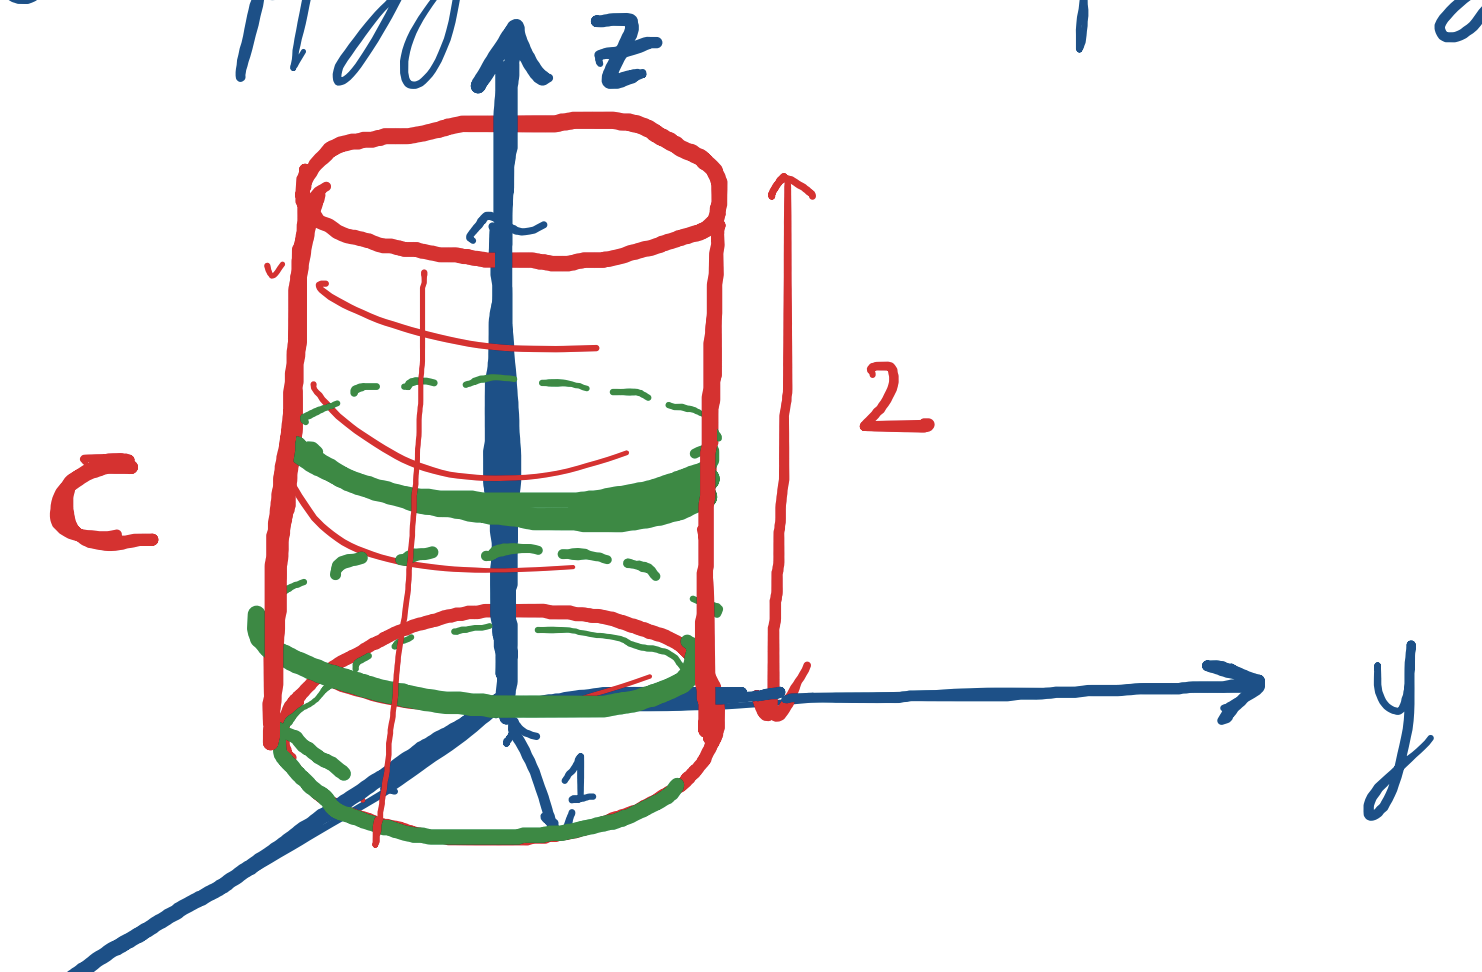
\includegraphics[width=4.5cm]{images/ess-legamu-defi.png}
\end{wrapfigure}
\hspace{-15pt}di base = 1, altezza = 2, e che si appoggi sul piano xy. 
\begin{itemize}
    \item Non possiamo descriverla come superficie cartesiana.
    \item Possiamo nemmeno descrivere il nostro cilindro come superficie implicita aggiungendo una limitazione, infatti dobbiamo vedere il cilindro come $C = \{(x,y,z) \in \mathbb{R}^3 \::\: x^2 + y^2 = 1, 0\leq z \leq 2\}$, riusciamo quindi a scriverlo come superficie implicita ma con una limitazioni ad una delle variabili ($0\lq z \leq 2$).
\end{itemize} 
\newpage
\begin{itemize}
    \item Possiamo scriverla anche come superficie parametrica, per farlo usiamo come parametri $z$ ed il $\Theta$ delle coordinate polari $(\rho \equiv 1$ perché la circonferenza di base ha raggio 1), quindi scriviamo $C = \{(x,y,z) \in \mathbb{R}^3 \::\: (x,y,z) = (\cos{\Theta}, \sin{\Theta}, z)\}$ con $\{0 \leq \Theta \leq 2\pi$ e $0\leq z \leq 2\}$.
\end{itemize}


\begin{example}
Partiamo da la semisfera di raggio 3 che sta sull'asse xy. Vediamo di descrivere le superficie.\\
\end{example}
\begin{wrapfigure}[6]{l}{5cm}
    \vspace{-25pt}
    \centering
    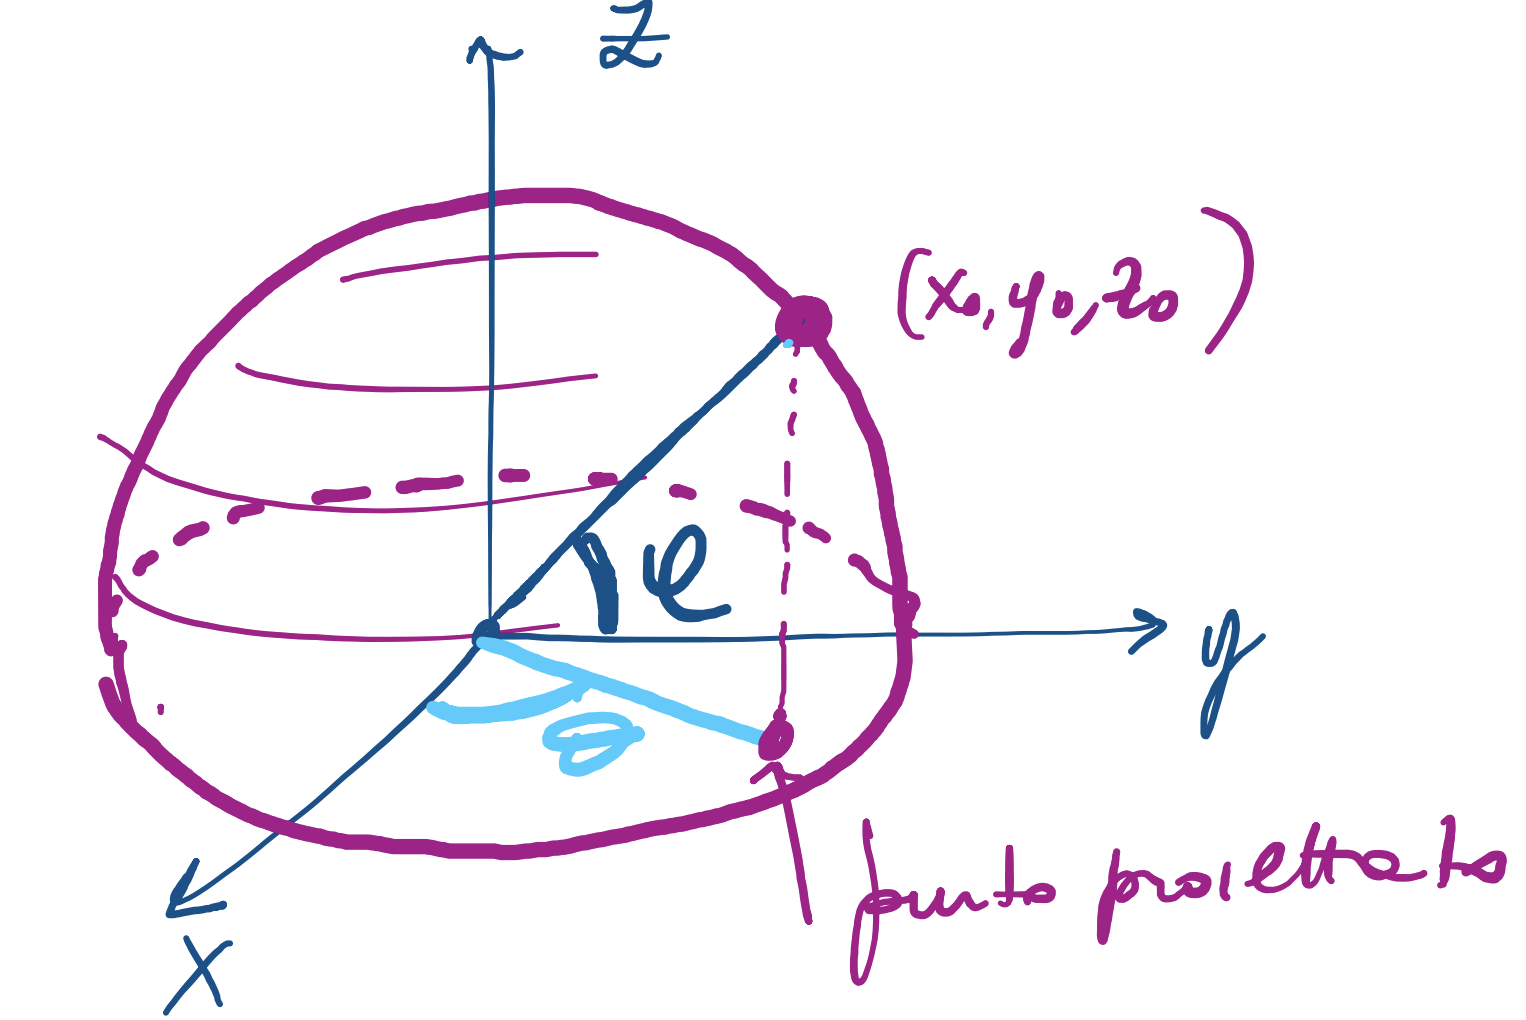
\includegraphics[width=4.5cm]{images/ess-legamu-defi-2.png}
\end{wrapfigure}
\hspace{-15pt}Possiamo descriverla come superficie parametrica usando le coordinate sferiche e mettendo $S = \{(3\cos{\Theta} \cdot \sin{\phi}, 3\sin{\Theta}\cdot\sin{\phi}, 3\sin{\Theta}\phi) \text{ con }0\leq \Theta \leq 2\pi, 0\leq \phi \leq \frac{\pi}{2}\}$, abbiamo che $3\cos{\Theta}, 3\sin{\Theta}$ sono le coordinate polari del punto proiettato sul piano xy, le 3 coordinate che escono sono le coordinate sferiche.\\\\


\hspace{-15pt}Vediamo ora, dopo aver descritto una superficie, di definire il piano tangente ad una superficie, ed il vettore normale ad una superficie (con vettore normale si intende il vettore perpendicolare al piano tangente). Prendiamo in considerazione una superficie cartesiana decritta dall'equazione $z = f(x,y)$, quindi $S = \{(x,y,z) \in \mathbb{R}^3 \::\: z = f(x,y)\}$, data questa superficie vediamo come scrivere il piano tangente nel punto $(x_0,y_0,f(x_0,y_=))$. \\\\
Sappiamo che possiamo scrivere $f(x_0 + h, y_0 + k) = f(x_0, y_0) + f_x(x_0,y_0) \cdot h + f_y(x_0,y_0) \cdot k + o(\sqrt{h^2 + k^2})$, dove $f(x_0, y_0) + f_x(x_0,y_0) \cdot h + f_y(x_0,y_0) \cdot k$ ci da l'equazione del piano tangente, se poniamo $x_0 + h = x$ e $y_0 + k = y$ possiamo sostituire ed otteniamo $h = x - x_0$ e$k = y - y_0$, quindi otteniamo $z = f(x_0,y_0) + f_x(x_0,y_0) \cdot (x-x_0) + f_y(x_0,y_0)(y-y_0)$ che è l'equazione del piano tangente.\\

\begin{wrapfigure}[7]{r}{5.3cm}
    \vspace{-10pt}
    \centering
    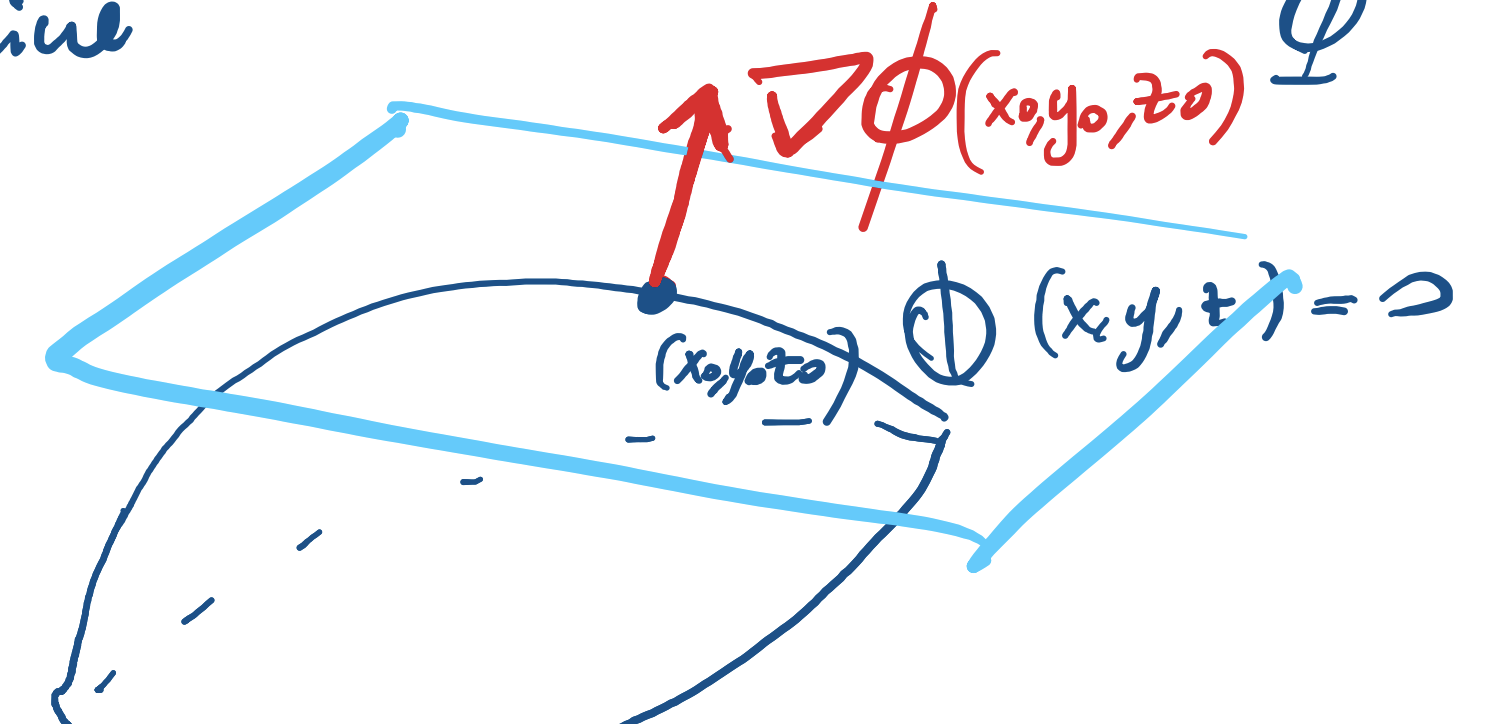
\includegraphics[width=4.5cm]{images/sup-implicita.png}
\end{wrapfigure}
Se invece partiamo da una superficie implicita quindi $s = \{(x,y,z) \in \mathbb{R}^3 \::\: \varphi(x,y,z) = 0\}$, in questo caso ci accorgiamo che il luogo di zeri, cioè S, è in realtà un insieme di livello per $\varphi \Longrightarrow$ S è perpendicolare al gradiente di $\varphi$. Quindi il piano tangente ad S in un punto $(x_0,y_0,z_0)$ è il piano che passa per $(x_0,y_0,z_0)$ ed è perpendicolare a $\nabla \varphi(x_0,y_0,z_0)$. Di conseguenza il piano ha equazione $(x,y,z) \in$ piano se $<\nabla \varphi(x_0,y_0,z_0),(x,y,z)> = d$ dove d è una costante scelta in modo che il piano passi per $(x_0,y_0,z_0)$. Quindi l'equazione $<\nabla \varphi(x_0,y_0,z_0),(x,y,z)> = d$ in modo esplicito diventa $\varphi_x (x_0,y_0,z_0) \cdot x + \varphi_y(x_0,y_0,z_0) \cdot y + \varphi_z(x_0,y_0,z_0) \cdot z = \varphi_x (x_0,y_0,z_0) \cdot x_0 + \varphi_y (x_0,y_0,z_0)y_0 + \varphi_z (x_0,y_0,z_0) \cdot x_0$.